\documentclass[a4paper,left=1.25cm,right=1.25cm,top=1.25cm,bottom=1.25cm]{article}
\usepackage{natbib}
\usepackage{amsmath}
\usepackage{caption}
\usepackage{placeins}
\usepackage{graphicx}
\usepackage{subcaption}
\usepackage{setspace}
\usepackage{float}

\usepackage{tikz}
\usetikzlibrary{arrows,calc,positioning,shapes.geometric}
\usepackage[left=1.25in,right=1.25in,top=1.25in,bottom=1.25in]{geometry}
%\usepackage[active,tightpage]{preview}

\usepackage{enumitem}
\setlist[description]{leftmargin=\parindent,labelindent=\parindent}
\bibpunct{(}{)}{,}{a}{}{;} 
\usepackage{url}
\usepackage{nth}
\usepackage{authblk}
% for the d in integrals
\newcommand{\dd}{\; \mathrm{d}}
\newcommand{\tc}{\quad\quad\text{,}}
\newcommand{\tp}{\quad\quad\text{.}}
\defcitealias{HMD}{HMD}

\newcommand\ackn[1]{%
  \begingroup
  \renewcommand\thefootnote{}\footnote{#1}%
  \addtocounter{footnote}{-1}%
  \endgroup
}

\newcommand{\absdiv}[1]{%
  \par\addvspace{.5\baselineskip}% adjust to suit
  \noindent\textbf{#1}\quad\ignorespaces
}
\begin{document}

\title{Alignment, clocking, and macro patterns of episodes in the life course}
\author[1,2,3]{Tim Riffe\thanks{tim.riffe@ehu.eus}}
\author[3]{Angelo Lorenti}
\author[3]{Andr\'{e}s Castro}
\affil[1]{Universidad del Pa\'{i}s Vasco}
\affil[2]{Ikerbasque (Basque Foundation for Science)}
\affil[3]{Max-Planck-Institute for Demographic Research}
\maketitle

\begin{abstract}

\absdiv{Background}Individuals are often observed passing through a sequence of discrete states in trajectory data. These are usually either simplified into transition probabilities to derive asymptotic values of aggregate statistics using Markov assumptions, or else retained for pattern and group detection using sequence analysis. Markov-derived aggregate statistics are of limited scope, and sequence analysis appears aimed at inferring typologies rather than generating demographic aggregates.
\absdiv{Objective}We propose a structured framework to generate novel aggregate demographic patterns and summary indices from trajectory data, including trajectories generated from Markov models by proposing a simple and extensible grammar of operations for trajectory data.
\absdiv{Methods}We introduce the concepts of clocking and alignment as a new framework for generating novel statistics from trajectories. 
\absdiv{Data}We use published transition probabilities to simulate discrete trajectories of employment states to demonstrate concepts. We use retrospective fertility and union trajectories from Colombian Demographic and Health Surveys data and disability trajectories simulated from European Statistics on Income and Living Conditions for Italy (EU-SILC) for example applications.
\absdiv{Results}We demonstrate  several new demographic aggregate patterns in the areas of disability inequalities and birth intervals.
\absdiv{Conclusions}We demonstrate the flexibility of this framework and the ease of generating macro patterns. An R package is provided to facilitate experimentation with these operations.
\end{abstract}

\doublespacing
\section{Introduction}

% Regularity in the age patterns of demographic rates often evoke 
% 
% Markov models
% 
% Sequence analysis aims to 
% 
% 
% Most of what we know about demography (levels, trends) stands on a Markovian foundation: The lifetable is a Markov process, as are most multistate models in practice, and these two analytic instruments underly what we know about longevity, healthy years lived, years worked, and many other of the primary concerns of demography. Results of this approach tend to be synthetic indices, a number or two to summarize an average lifetime from a possibly rich set of age-structured demographic rates or probabilities. And age-structured rates are already an abstraction from an even richer sequence of events and states. Moment statistics, such as life expectancy, are useful metrics, but we're not so sure that they
We propose a measurement framework consisting in a two-element grammar that helps to extract macro patterns hidden within trajectory data. Such patterns might be age-like patterns of novel prevalence, aggregates based on episodes of a given state, or other synthetic aggregates that might complement the reporting of state expectancies. Using this framework, we aim to zoom in on demographic patterns that emerge at various stages of the life course, and so describe a given demographic phenomenon (state) from a variety of perspectives. 

We first define \emph{clock} measures, a way to inscribe time, order, prevalence, or other measures into individual life trajectories. This step is partly analogous to defining a rewards matrix in multistate Markov models \citep[see e.g.][]{caswell2018matrix}. As an example of a concrete Markov analogy, \citet{dudel2018expanding} provides an algebraic expression to calculate the distribution of time spent within a given state in a multistate model. That approach can also be extended to produce age patterns of these distributions. Measures such as this (only reported once before to our knowledge \citep{laditka1998new}) are a subset of possible \emph{clock} measures. Clock measures are flexible, and enable the researcher to decompose expected episode durations into expected time spent and left within individual episodes of a state, or even by episode length. To illustrate the flexibility of \emph{clocks}, we propose several other clock variants that go beyond this case.

Second we define \emph{alignment} operations, which shift trajectories to have synchronous timing with respect to the entry to or exit from a given episode of a specified state. Researchers already do similar things: for example \citet{iacobelli2013multiple} propose a flexible use of time-since-event scales, and \citet{riffe2017unified} define Lexis spaces in which life lines are aligned both on birth and on death. Such approaches have been used to reveal hidden health patterns \citep{riffe2016time} and pathways \citep{potente2018disability, raab2018pathways}. We propose more flexible alignment procedures, which allow trajectory synchronization on the start or end of a conditionally specified episode, for example the first, last, or longest episode of a state.

Applied separately or in combination, clock and alignment operations open a large space for the derivation of demographic macro patterns. In the following sections we use a small simulation of old-age employment trajectories to illustrate concepts. We then give two abbreviated example applications for the cases of disability inequalities in Italy and birth interval differentials in Colombia. Disability trajectories are simulated from transition probabilities estimated from Italian EU-SILC data \citep{SILC}. Birth and union histories are self-reported retrospective histories from the Colombian Demographic and Health surveys. We conduct a few illustrative analyses of these data using the framework, which allows us to make new and interpretable comparisons. These introductory examples demonstrate the flexibility of the clocks and alignment framework for aggregations of trajectory data. Work shown here is fully reproducible, and we also offer an experimental package, \texttt{Spells} in the open source \texttt{R} programming language \citep{r2020}, which enables readers to easily apply flexible clock and alignment operations.
% 
% Incidence-based matrix models are rather undeveloped with respect to tenure-statistics, and these might be of interest for a variety of substantive reasons. By tenure statistics I refer to the statistics of particular spells or episodes of a state. For example, in incidence-based models with bidirectional flows (i.e., allowing for recovery and then re-onset, and so on), modelled individuals may pass through a state, such as sickness, many times before death. Typically a transition matrix manipulation would only give us the average time spent sick or moment statistics thereof. Recently matrix calculations have been described for how to calculate the average number of episodes of a given state \citep{dudel2017b}. Combined with the average state occupancy, this information yields the average duration of episodes.

% One may wonder how the average spell duration changes with age, and for this there is no ready matrix expression. Such analytic expressions are surely possible, but in the following I intend to propose a suite of operations (including the aforementioned) so broad and flexible as to fill the lifetime of a matrix buff. I proceed using simulations rather than matrix calculations because it will save the work of deriving and checking dozens of formulas. In this way, we have the liberty to change definitions without incurring methodological setbacks. Since we simulate, we get stochastic stationary distributions of each measurement for free, which I'll represent using fan-chart visualizations. This approach is not all that different from that proposed by \citet{laditka1998new}, but I expand on their approach by proposing a set of count statistics called \emph{clocks} and age \emph{realignments}, which together result in a large (unbounded?) set of age-like patterns of state episodes. These same operations can be used on observed populations of sequences as well, but the key difference is that observed populations are not stationary. Our example will refer to the stationary tenure statistics that belong to a particular set of age-specific transition rates, although the configuration of transition rates used to generate results is immaterial.

\section{Concepts}

\subsection{Definitions}

A life sequence can be represented as an ordered set of discrete states observed over time. Given a sequence of possible states, we refer to contiguous observations or runs of a given state as spells. A spell of a given state consists in a certain number of time steps, covering some total duration of elapsed time \citep{cornwell2015}. We define clocks and alignments as operations that map the elements of life sequences to new sequence measures conditional upon the episode structure. More specifically,

\begin{description}
    \item[Reference state] is the state to which a statistic refers. For example, the reference state for working life expectancy is \emph{employment}.
    \item[Clocking] operations assign new time step or spell order values to positions within spells of a specified reference state conditional upon the structure of the reference state within the sequence.  
    \item[Alignment] is a uniform shift of the timeline of a sequence such that the position of the time origin is conditional on spells of a reference state within the sequence. 
\end{description}

It may help to imagine clocks and alignments as functional mappings of paired sequence and timeline sets to output that follows the same positional order.

\subsection{Example data}
To illustrate clock and alignment concepts, we simulate sequences from a published transition matrix \citep{Dudel2017}. This matrix refers to black women in the USA aged 50-100 in 1994, and it contains age-structured transition probabilities for movements between employment, inactivity, and retirement, as well as mortality from these three states, all estimated from the US Health and Retirement Study \citep{HRS}. Simulation is done using the \texttt{rmarkovchain()} function from the \texttt{R} package \texttt{markovchain} \citep{spedicato2017}. A glimpse of 10 randomly generated individuals is shown in Figure~\ref{fig:seq10}.  Each trajectory begins in a state of employment at age 50 and ends in death.

\begin{figure}[ht!]
\centering
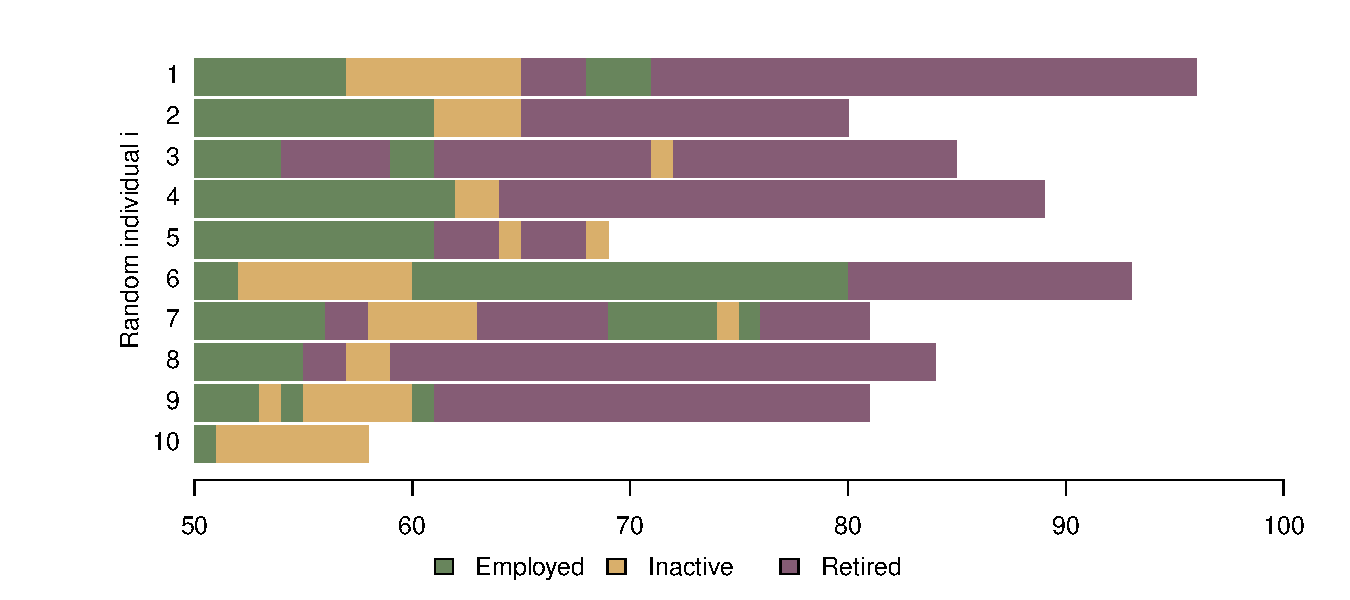
\includegraphics[scale=.5]{Figures/Seq10.pdf}
\caption{Ten randomly generated state sequences from the 1994 transition matrix
of black females \citep{Dudel2017}}
\label{fig:seq10}
\end{figure}

 In the following, imagine this visualization as an array, with individuals in rows and time steps in columns. Ages after death may just be imputed with \texttt{NA} to ensure a rectangular table. Practically, an array representation of trajectories is not required, and all operations we define work identically in either array or \texttt{tidy} programming approaches \citep{wickham2014tidy}.

\FloatBarrier

\subsection{Clocks}
\label{sec:clocks}

\subsubsection{Prevalence as a simple case}
Prevalence is defined as the fraction of individuals in each time step that are in a reference state. Calculations of prevalence in this setup proceed by imputing reference states with 1s (with 0s elsewhere) and calculating column means over survivors in each age. Figure~\ref{fig:seq10ones} represents such a data construct, where the state sequence matrix has been converted to a binary matrix, with 1s for employment episodes, 0s for other living states (shown blank). As the number of simulated trajectories increases, the resulting age pattern of prevalence will approach the values in the respective column of the so-called fundamental matrix in a Markov approach \citep{caswell2018matrix}.

\begin{figure}[ht!]
\centering
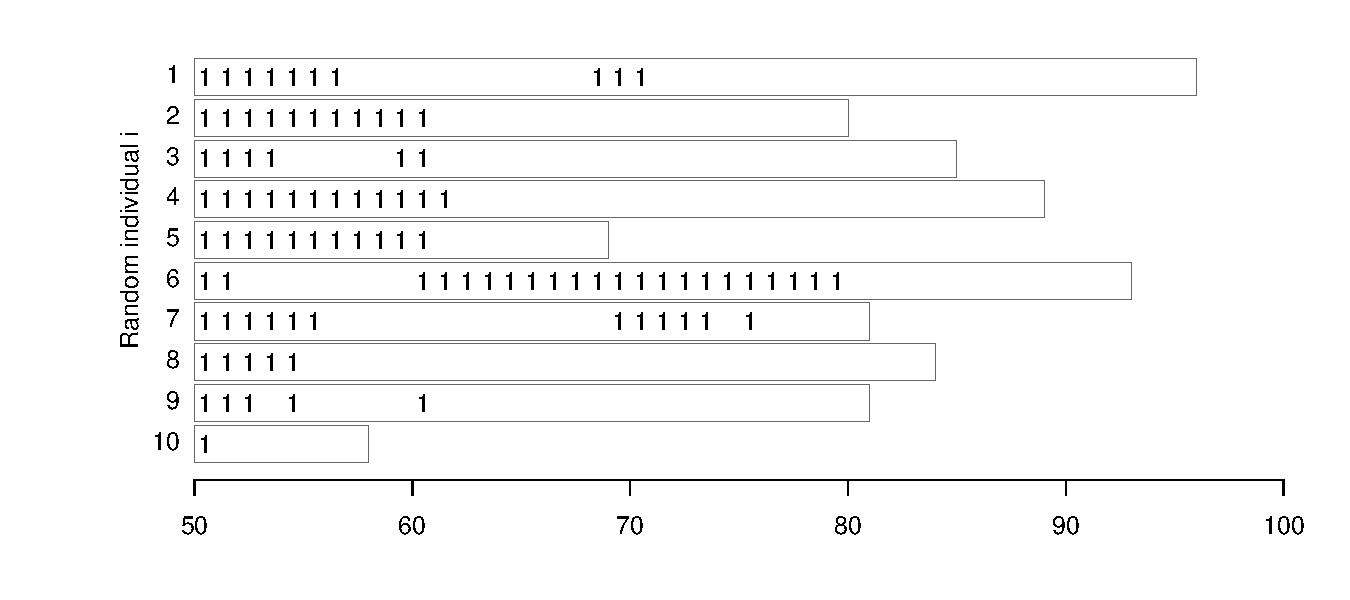
\includegraphics[scale=.5]{Figures/Seq10ones.pdf}
\caption{Binary imputation of employment spells}
\label{fig:seq10ones}
\end{figure}

\subsubsection{Duration, step, and order clocks}
To derive aggregate measures other than prevalence, change the 1s in Fig.~\ref{fig:seq10ones} to other values. For example, to calculate an age-pattern of inactivity episode duration, create an array where each time step of the inactivity state is imputed with values equal to the total episode length (Fig.~\ref{fig:seq10dur}). Such a calculation is conditional on being in an episode of the reference state, such that values outside the reference state are ignored when producing summary statistics. Column means of the duration-mapped array would give the average episode duration conditional on being in the reference state. 
To condition spell duration on episodes starting (ending) in each age, instead impute the episode duration values in only the first (last) time step within each episode (not shown). To calculate time spent or left in the state episode, per Fig.~\ref{fig:seq10timespent} or \ref{fig:seq10timeleft} \footnote{In practice we may increment values by $\frac{1}{2}$ a time interval to imply mid-interval time references.}. Episodes can also be imputed with other markers, such as episode order, as in Fig.~\ref{fig:order} for the case of employment spells, or episode fractions. 

\begin{figure}[ht!]
\centering

\begin{subfigure}{\textwidth}
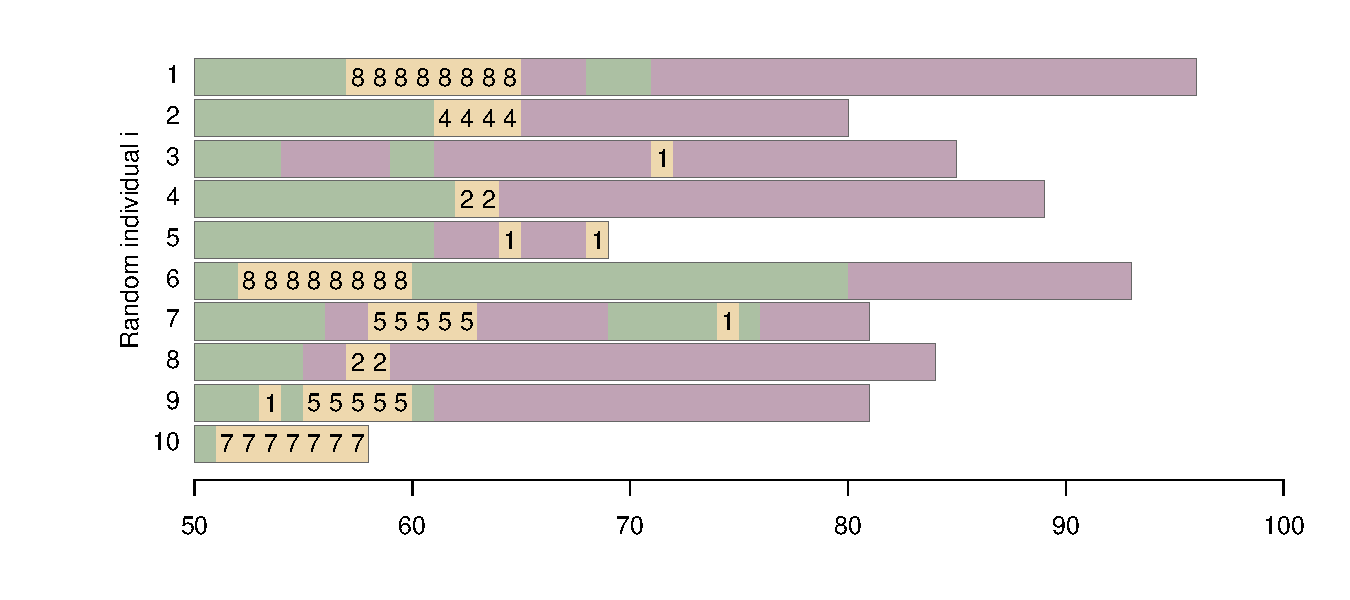
\includegraphics[scale=.5]{Figures/Seq10dur.pdf}
\caption{Static; Total episode duration of inactivity.}
\label{fig:seq10dur}
\end{subfigure}

\begin{subfigure}{\textwidth}
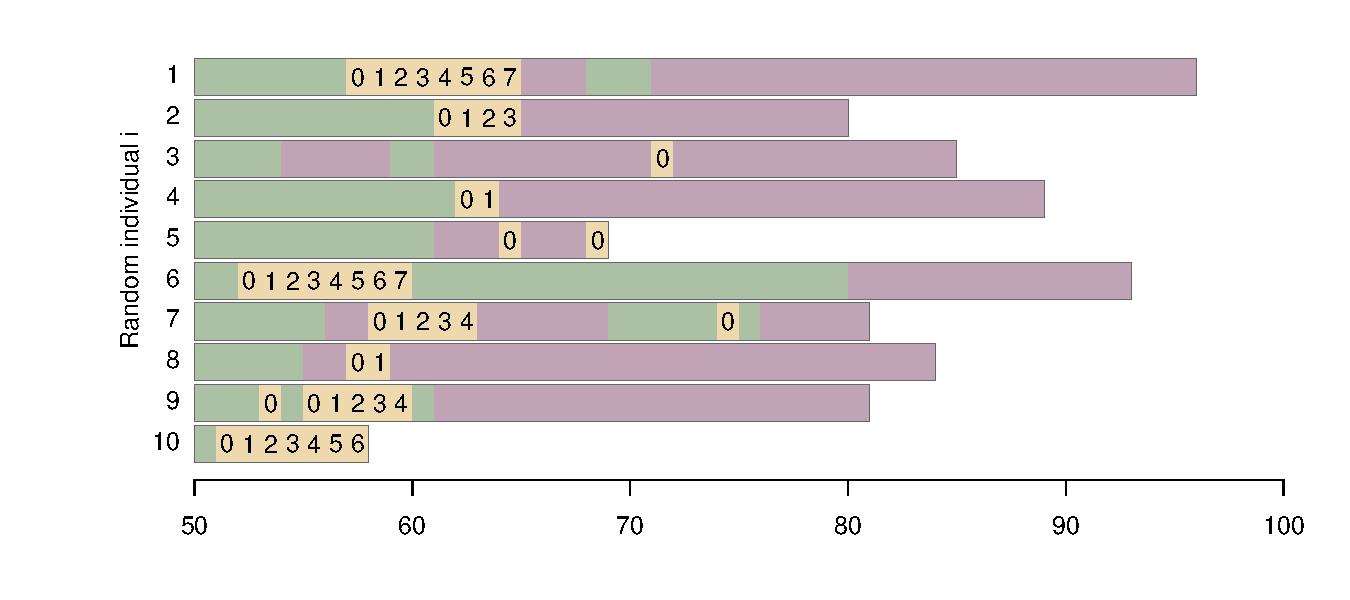
\includegraphics[scale=.5]{Figures/Seq10timespent.pdf}
\caption{Step; Time spent in episode of inactivity.}
\label{fig:seq10timespent}
\end{subfigure}

\begin{subfigure}{\textwidth}
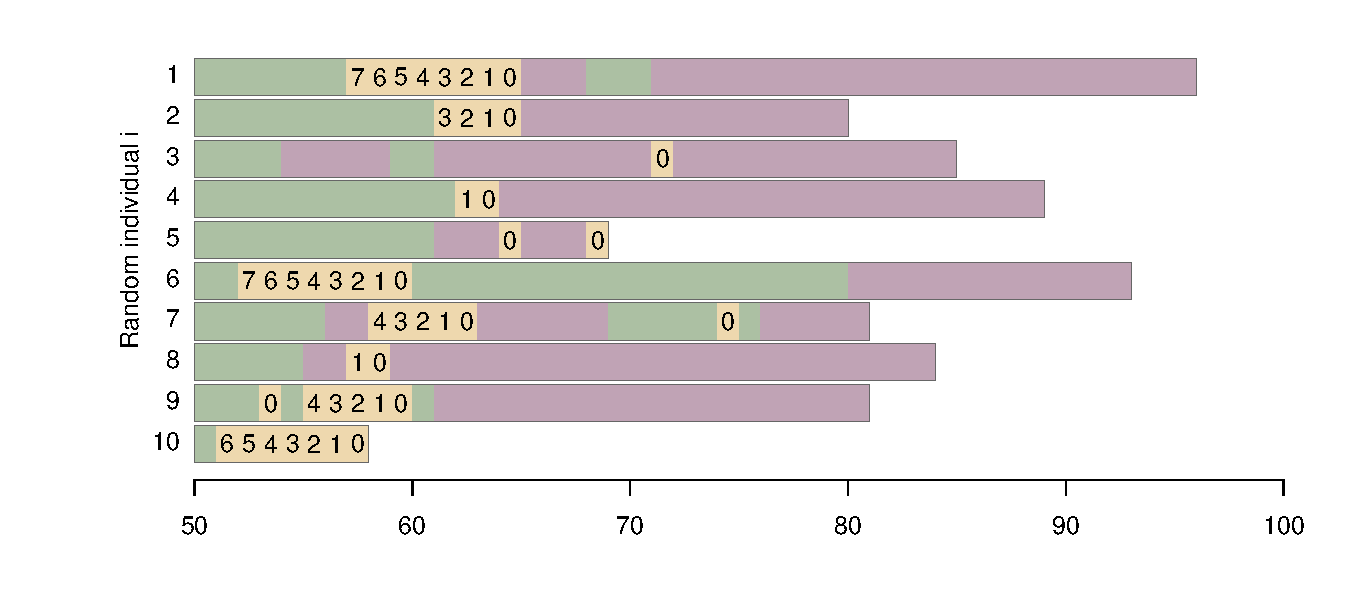
\includegraphics[scale=.5]{Figures/Seq10timeleft.pdf}
\caption{Step; Time left in episode of inactivity}
\label{fig:seq10timeleft}
\end{subfigure}
\caption{Inactivity spells from Figure~\ref{fig:seq10}
are imputed with duration and step clocks.}
\label{fig:spentleft}
\end{figure}

\begin{figure}[ht!]
\centering

\begin{subfigure}{\textwidth}
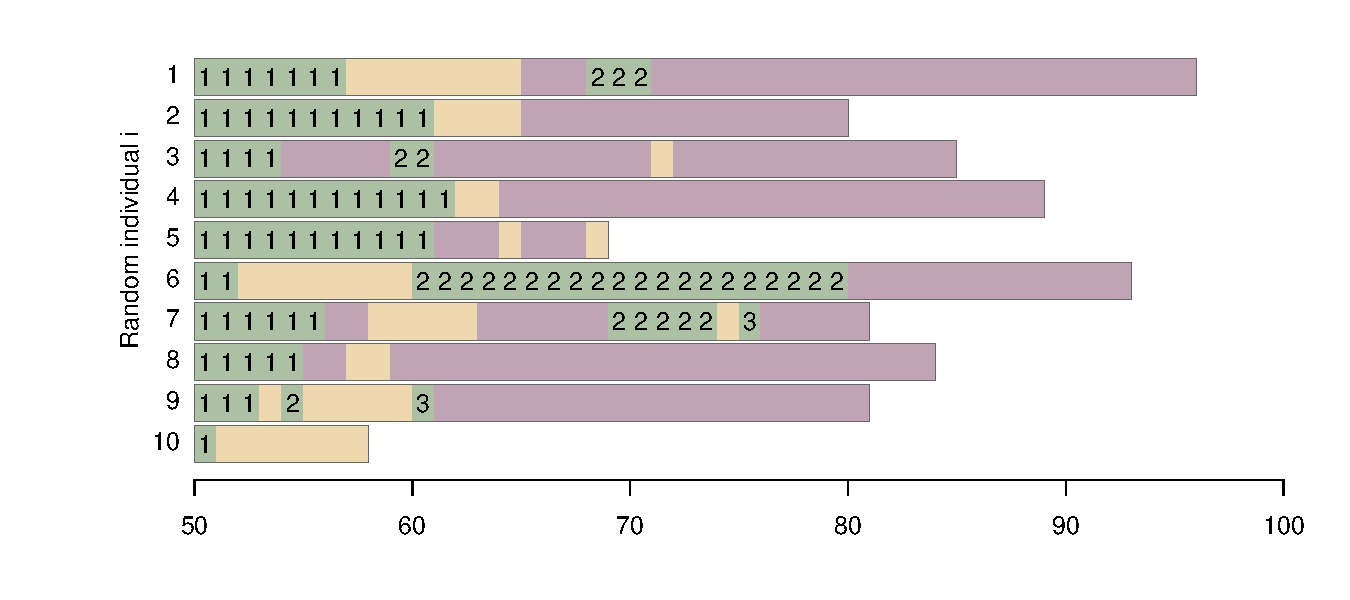
\includegraphics[scale=.5]{Figures/Seq10ordUp.pdf}
\caption{Employment episode order, increasing.}
\label{fig:orderup}
\end{subfigure}

\begin{subfigure}{\textwidth}
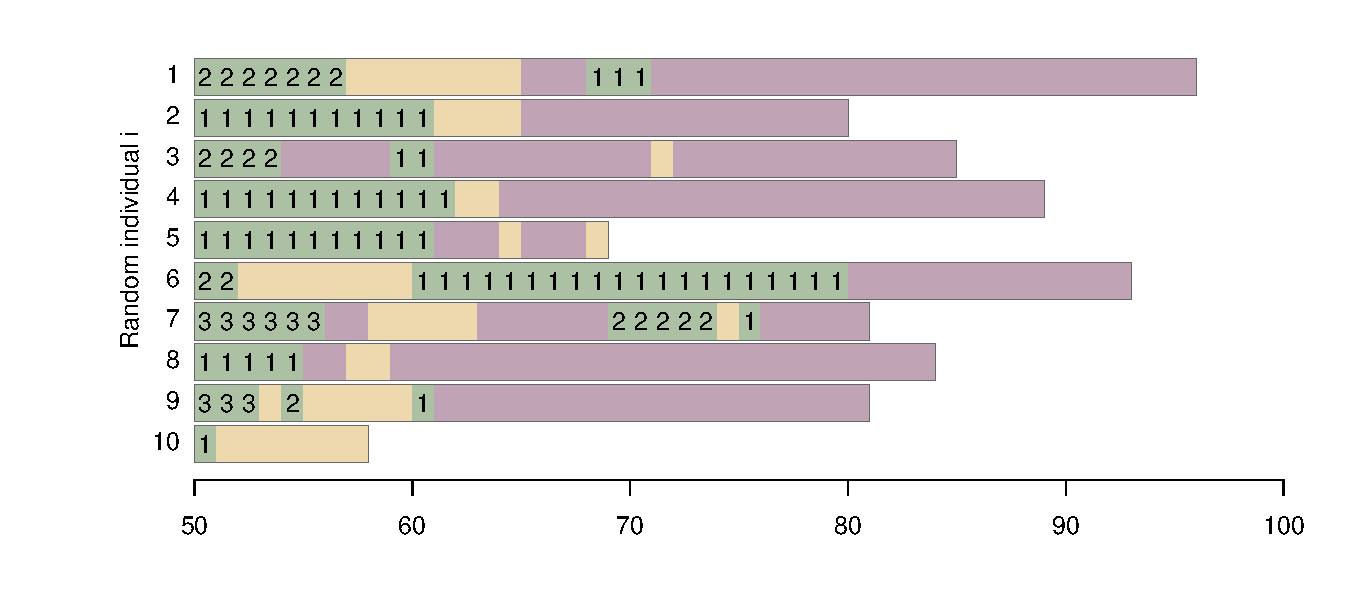
\includegraphics[scale=.5]{Figures/Seq10ordDown.pdf}
\caption{Employment episode order, decreasing.}
\label{fig:orderdown}
\end{subfigure}

\caption{Employment episodes from Figure~\ref{fig:seq10}
are imputed with order count variables.}
\label{fig:order}
\end{figure}

There is room for creativity in defining clock measures such as these, and we encourage experimentation along these lines. Clock measures follow simple rules of construction, but aggregation within time intervals may result in patterns that are difficult to foresee. The clocks shown in Figs.~\ref{fig:spentleft} and \ref{fig:order} are aligned on age, such that direct aggregation (column operations) would result in age patterns.  One may wish to synchronize trajectories in ways other than age, thereby defining a different time structure that results in a different macro pattern after aggregation.

\FloatBarrier
\subsection{Alignment}
\label{sec:align}
Episodic \emph{clock} values are aggregated according to some structuring criterion. In Figs~\ref{fig:seq10}-\ref{fig:order} the structuring criteria is chronological age, which is how data were generated in the first instance. To introduce a term, the sequences in these figures are \emph{left-aligned} on the event of birth. This is the most common default alignment in social and medical sciences, but other choices may be more compelling for particular questions.

For older-age processes, birth is decades away from the events and states of interest, and sharper and perhaps more regular patterns may be be found with respect to other alignment criteria. Aligning lifelines requires selecting i) a reference moment or anchoring \emph{event} , and ii) an alignment direction. A reference event could be any instance of entry, exit, or other compelling anchor point, such as a spell midpoint; such events may relate to episodes themselves. For repeated events, the choice of anchoring episode could itself follow a regular criterion, such as first, last, or longest episode. The \emph{direction} of alignment could be left, right, center, or perhaps something else.

Fig.~\ref{fig:alignment} shows a set of four alignment selections out of the
many possible choices. Fig.~\ref{fig:firstretire} left-aligns on
entry to \emph{first} retirement (if any). One could also choose last, longest,
or some other episode of retirement, or of course right-align on exit.
Fig.~\ref{fig:longinactleft} left-aligns on entry into each individual's
longest spell of inactivity, whereas Fig.~\ref{fig:longinactright} right-aligns on exit from
the same spell.

 \begin{figure}[ht!]
\centering
\caption{The sequences from Figure~\ref{fig:seq10} under a variety of alignment
types.}
\label{fig:alignment}

\begin{subfigure}{\textwidth}
\centering
\caption{Right-aligned on death.}
\label{fig:seq10death}
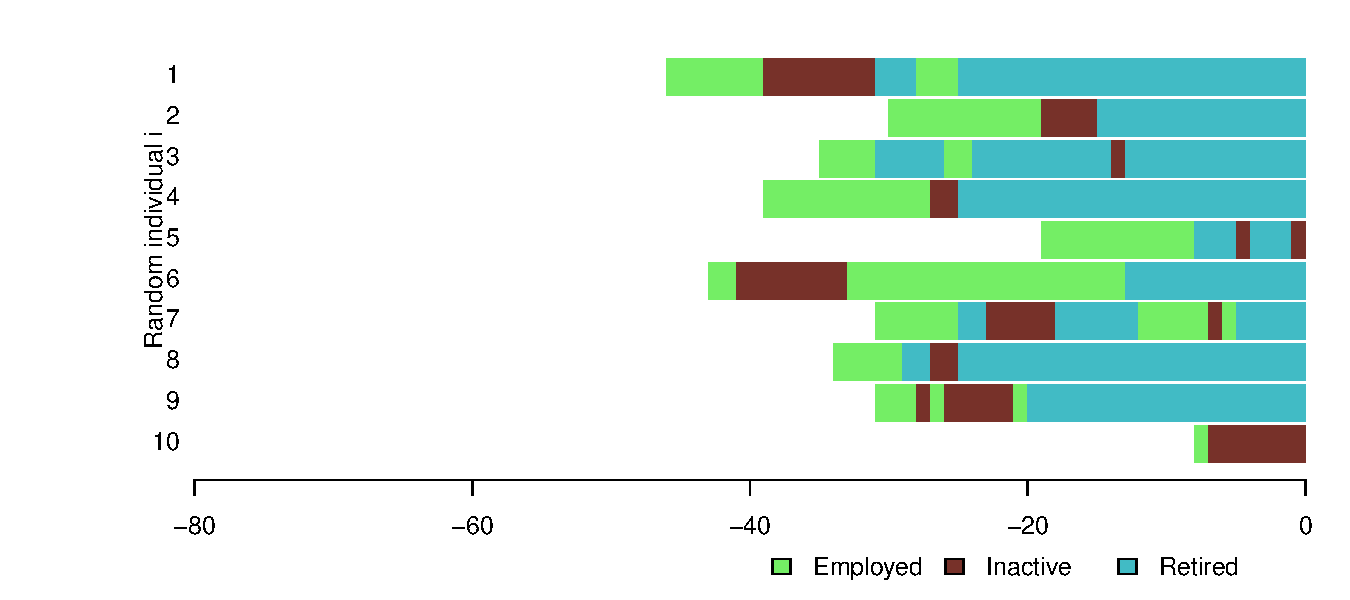
\includegraphics[scale=.5]{Figures/Seq10deathalign.pdf}
\end{subfigure}

\begin{subfigure}{\textwidth}
\centering
\caption{Left-aligned on \emph{first} retirement.}
\label{fig:firstretire}
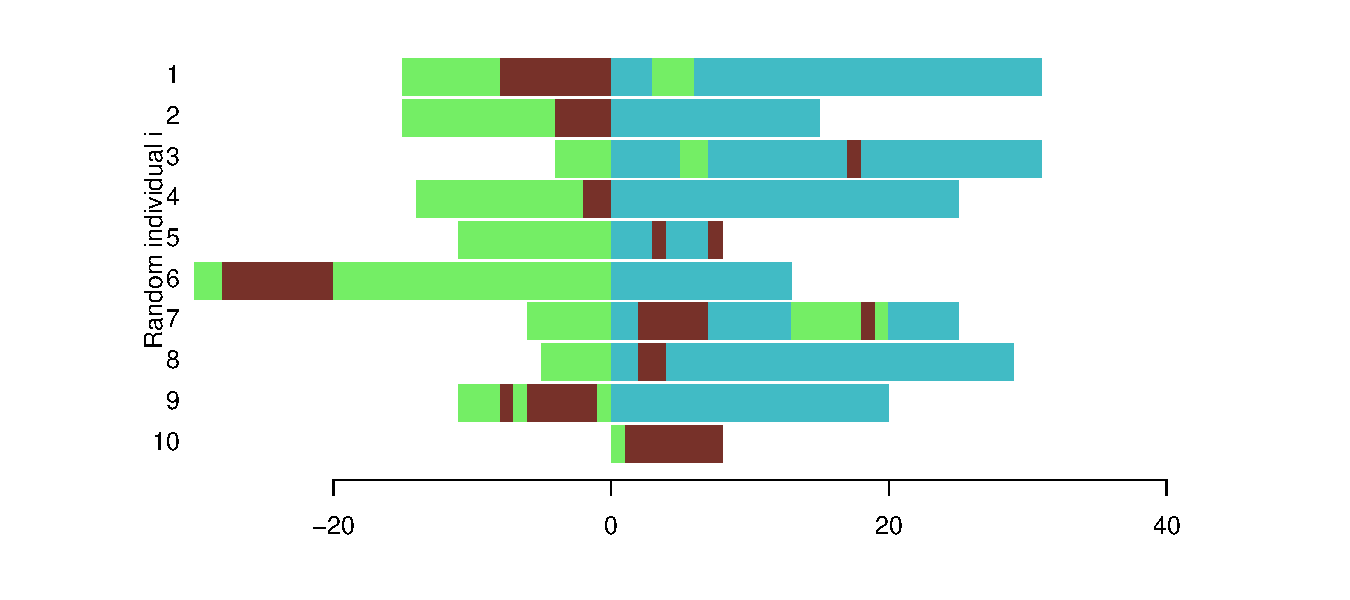
\includegraphics[scale=.5]{Figures/Seq10firstretirealign.pdf}
\end{subfigure}

\begin{subfigure}{\textwidth}
\centering
\caption{Left-aligned on entrance to \emph{longest} spell of inactivity}
\label{fig:longinactleft}
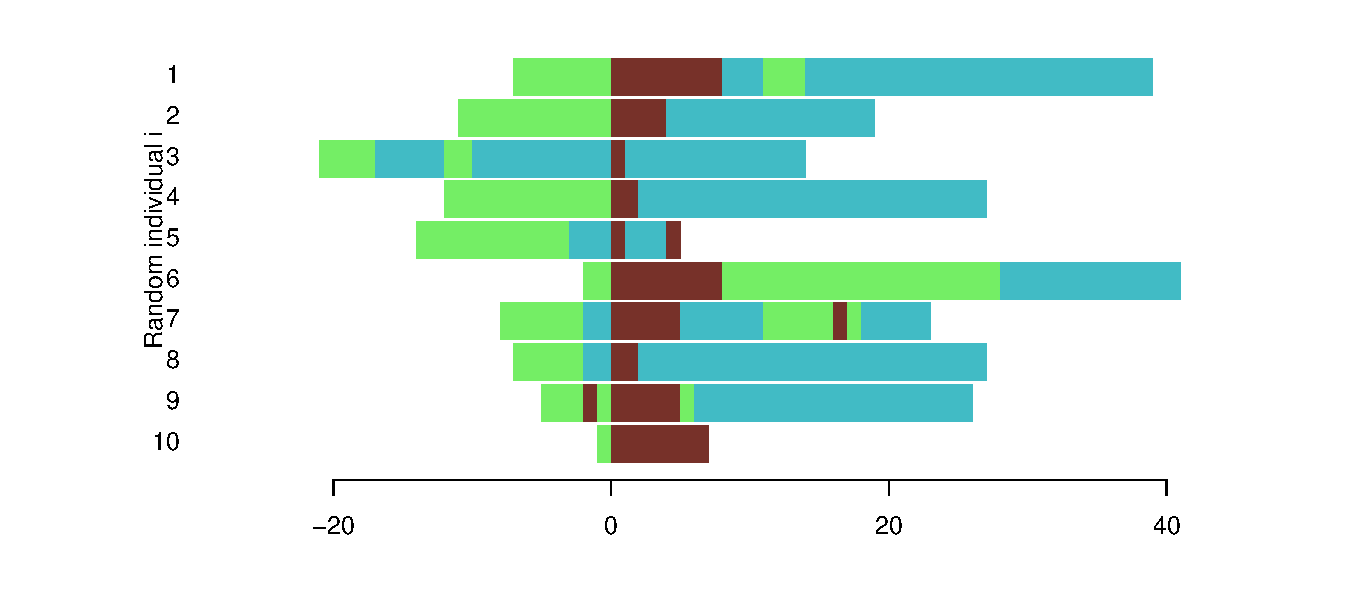
\includegraphics[scale=.5]{Figures/Seq10inactlongleft.pdf}
\end{subfigure}

\begin{subfigure}{\textwidth}
\centering
\caption{Right-aligned on exit from \emph{longest} spell of inactivity}
\label{fig:longinactright}
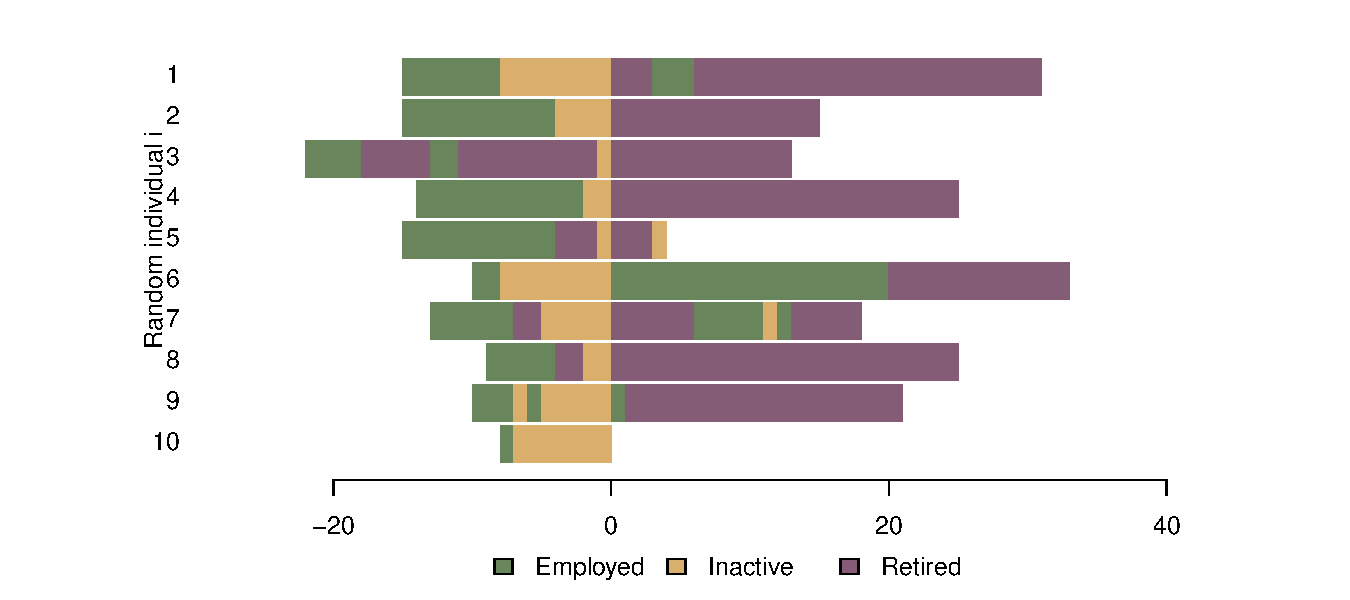
\includegraphics[scale=.5]{Figures/Seq10inactlongright.pdf}
\end{subfigure}

\end{figure}

These examples are subset of many possible alignments, in this case column shifting within rows of a matrix. Further, although we demonstrate concepts by visualizing hypothetical state sequences, alignment as shown here is unlikely to reveal patterns when directly visualizing raw trajectories. The researcher would probably want to define \emph{sort} operations (row-swapping) for this, or other visual abstraction techniques such as those proposed by \citet[e.g.][]{fasang2014visualizing}. In the present, we instead aggregate alignments and clocks to derive .

\FloatBarrier
\subsection{Trajectory aggregation}
Macro-demographic patterns are derived from trajectory data by aggregating clocks within time intervals. Aggregated clocks could assume any of the varied forms discussed here, or others. Discrete time intervals may draw from the original time scale, for example chronological age, or they may correspond to the structured results of an alignment operation, or a higher-dimensional cross-tabulation of time measures. Aggregation could be any functional mapping of the distribution of clocks within in a given time bin to a synthetic result. In our applications, we calculate means or quantiles of selected clocks.

The following section presents two examples where clocks and alignment operations are used to examine trajectory data. In the first example we rely on an ascending step clock measures and the standard age alignment to produce a disability spell pattern. In the second example we use three clocks and one alignment operation to study the mean duration of birth intervals according to the age of the mother at first birth, and the sex of the first child.

\section{Applications}

\subsection{Health inequalities}
Population level studies of disability typically report values such as mean time spent disabled, either derived from a multistate model of disability \citep{crimmins2009change} or derived using the Sullivan method \citep{Sullivan1970,Crimmins1997}. It is rare to see other model statistics reported for health disparities \citep{laditka1998new}, even for results based on simulated disability trajectories. Especially for the case of understanding group inequalities, it is valuable to measure quantities beyond health expectancies, such as the age pattern of disability spell length, or the extent to which disability is spread throughout life or concentrated at the end of life. Do new bouts of disability tend to get longer or shorter with age? Who has longer spells of disability, the rich or the poor? We demonstrate some basic clock and alignment operations that enable the calculation of age patterns for i) disability spell duration, ii) disability spell order, and iii) the prevalence of disability in the final years of life.

Long term disability trajectories over the life course of individuals are typically not recorded, except in rare cohort studies, or in long-running health registers. To produce our base set of trajectories, we first estimate transition probabilities, then we simulate over a wide age range. Each of our three measures demonstrates the results of a particular combination of clock and/or alignment operations.

\subsubsection{Data}
We use the Italian survey of the EU-SILC (European Statistics on Income and Living Condition), 2012-2015. The EU-SILC is the European Union (EU) reference source for comparative statistics on income and living conditions for all the countries in the EU. Member States conduct the survey annually, collecting nationally representative household and personal data. There is a cross-sectional and a longitudinal component. The longitudinal Italian EU-SILC is based on the rotational design proposed by Eurostat; each year, a new sample representative of the whole Italian population enters the study, and it is followed for four years. In the initial year, the sample is representative of the population 14 years old and over; for individuals aged over 80, the exact age is not made available in the data.

We use data for individuals who were first interviewed in 2012, 2013, and 2014 and re-interviewed in subsequent years. Thus, in our data, we have 29,570 individuals, 14,384 men and 15,186 women, followed over two, three, or four consecutive years.  

To estimate the transition probabilities between healthy and disabled states, refer to functional limitations, as measured with the question: ``for at least the past six months, to what extent have you been limited because of a health problem in activities people usually do?'' Possible responses are: ``Severely limited'', ``Limited but not severely'', and ``Not limited at all''. We aggregate ``Severely Limited'' and ``Limited but not Severely'' into a single category, ``Disabled'', and the remaining options into ``Healthy''. For respondents lost to the follow-up, information about death is provided by other household members.

Individuals aged 15 can be healthy or disabled, and those who survive up to age 16 can stay healthy or move to the disabled state; the process continues at each successive age, up to 79. The state space and valid transitions for this model are depicted in Fig.~\ref{fig:statespace}.

\begin{figure}[t!]\centering
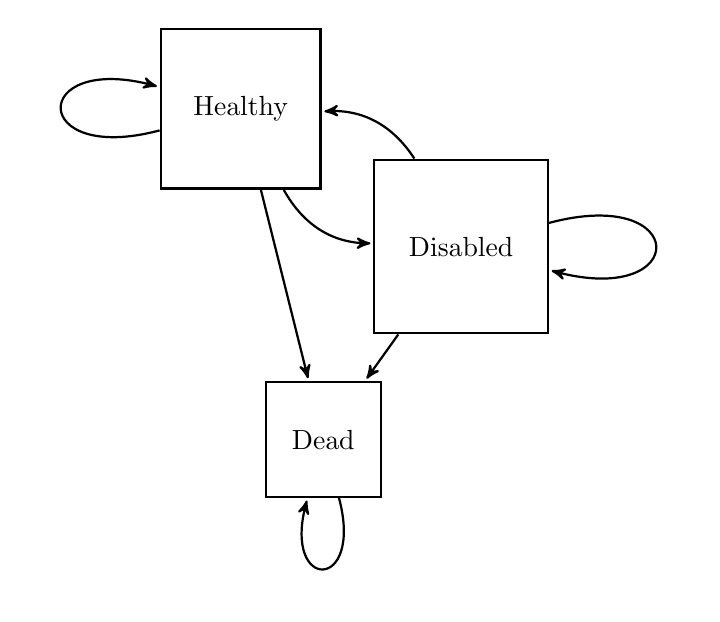
\begin{tikzpicture}[scale=0.7, ->,>=stealth',shorten >=1pt,auto,node distance=3.5cm,
  thick,main node/.style={circle,draw},square/.style={regular polygon,regular polygon sides=4}]

  \node[main node] (1) at (0,0) [square,draw]{Healthy};
  \node[main node] (2) at (4,-2.5) [square,draw] {Disabled};
  \node[main node] (3) at (1.5,-6) [square,draw] {Dead};  

  \path[every node/.style={font=\sffamily\small}]
    
    (1) edge node [left] {} (3)
   	 (1) edge [bend right] node [left] {} (2)
    
    (2) edge node [right] {} (3)
       (2) edge [bend right] node [left] {} (1)
    
    (1) edge [loop left] node {} (1)
    (2) edge [loop right] node {} (2)
    (3) edge [loop below] node {} (3)
 
    ;
\end{tikzpicture}
%\caption{Simplified state space of the healthy LE ignoring age.}\label{fig:state1}
\caption{A state space diagram depicting states and transitions for a single age step. States are in boxes and valid transitions are shown as arrows.}
\label{fig:statespace}
\end{figure}

We estimate the transition probabilities using multinomial regression \citep{Allison1982}. We model the probability of being in state $j$ (Healthy, Disabled, Dead) at time $t + 1$ as a function of the state $i$ at time $t$ (Healthy, Disabled) and age and income quintiles, separately by sex. In each of the regressions, age is modelled as a cubic spline. This approach accounts for non-linearity in the relationship between age and the probability of being in a state $i$. For each sex and income quintile, we produce transition probabilities $p_{i,j}$ for 65 age groups (single ages 15 to 79), and 6 possible transitions.

We arrange transition probabilities into standard Markov transition matrices, and then simulate 50,000 trajectories using the \texttt{rmarkovchain} package \citep{spedicato2017} and assuming that everyone starts healthy at age 15. Each trajectory consists in 65 age steps, padded with ``Dead'' after deaths. 

We estimate percentile bootstrap confidence intervals for transition probabilities based on 1000 replications \citep{Cameron2005}.
To maintain the complex survey structure of the data, we resample health and life trajectories at the individual level from three subsets of individuals. One set for individuals interviewed for two waves, one for those interviewed for three waves, and one for those interviewed for four waves. The three sub-sets are combined into a complete set reflecting size and composition of the original sample. Sampling weights are used in the resampling procedure and in the regression models. 

\subsubsection{Grammatical operations}
We report three kinds of results for this application, which aim to illustrate the leverage that can be obtained from isolated clock or alignment operations. These include two clocks (spell duration and order), and one alignment (end of life). We illustrate the meaning of these operations using ten randomly generated trajectories left truncated at age 50 and conditioned on death before age 80. In order to calculate the mean duration of spells starting in age $x$, we record the spell duration in the first time step of each disability spell, following the pattern in Fig.~\ref{fig:a1g2}. This first analysis requires only a single clock step because we retain the default age alignment. Calculation of the mean conditional spell order (Fig.~\ref{fig:a1g2}) is based on a similar setup, with an order indicator imputed in the first time step. These first two clocks are to be aggregated as conditional means (conditional on entering the spell in a given age), so all other values (healthy, dead, later time steps in the same spell) are discarded. The third analysis aims to compare disability prevalence patterns in the final years of life (Fig.~\ref{fig:a1g3}). This is based on i) an \emph{identity} clock, which places 1s in each time step within disability spells and 0s in time steps spent healthy, and ii) alignment on the end of life.

\begin{figure}
    \centering
    \begin{subfigure}{\textwidth}
      \centering
    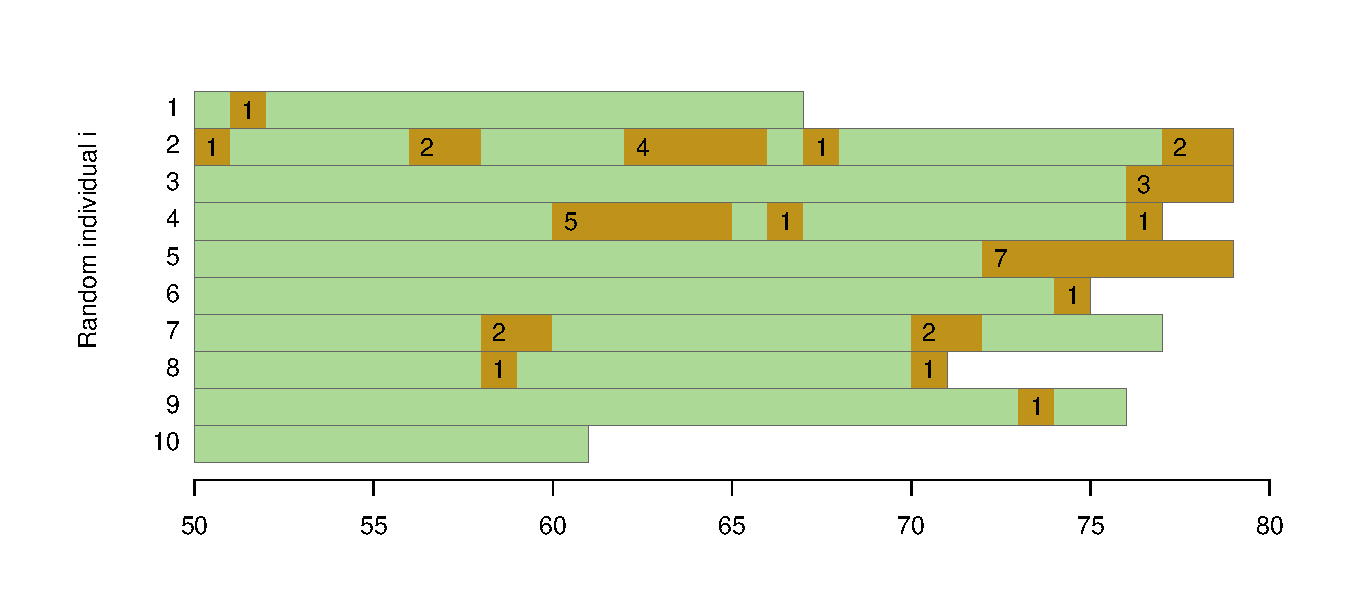
\includegraphics[scale=.45]{Figures/App1_grammar1.pdf}
    \caption{The first time step in each disability spell is imputed with the spell length, all other values are thrown out.}
    \label{fig:a1g1}
    \end{subfigure}
    
        \begin{subfigure}{\textwidth}
          \centering
    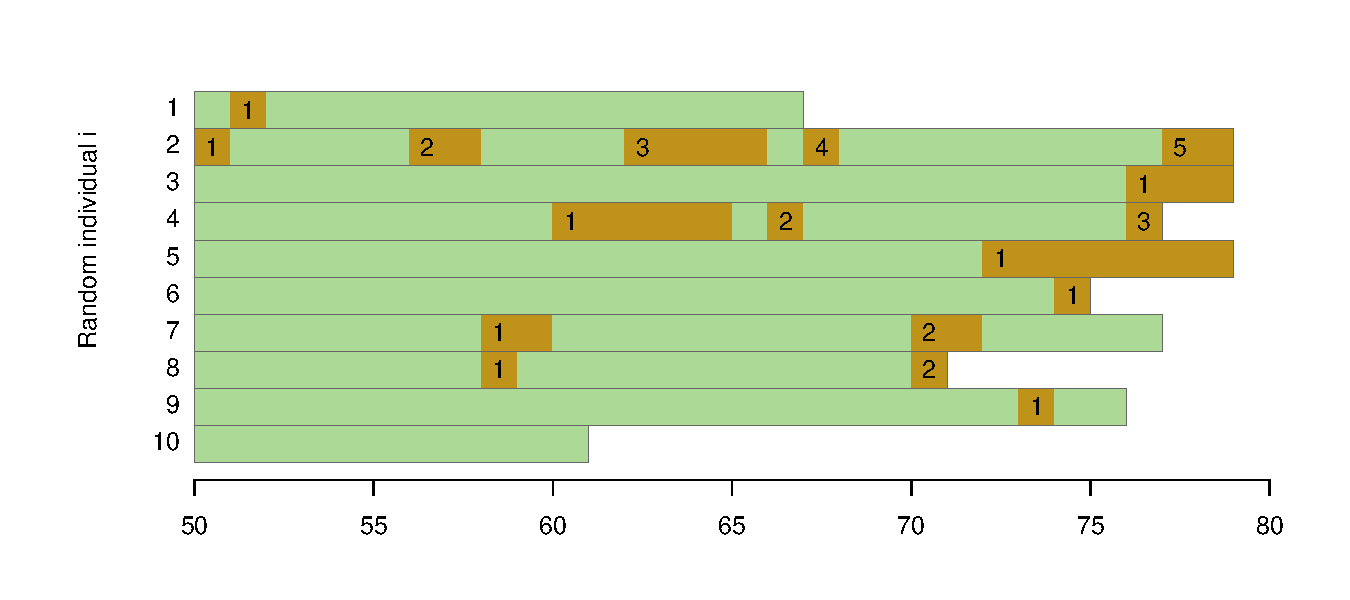
\includegraphics[scale=.45]{Figures/App1_grammar2.pdf}
    \caption{The first time step in each disability spell is imputed with an ascending spell order clock, all other values are thrown out.}
    \label{fig:a1g2}
    \end{subfigure}
    
        \begin{subfigure}{\textwidth}
          \centering
          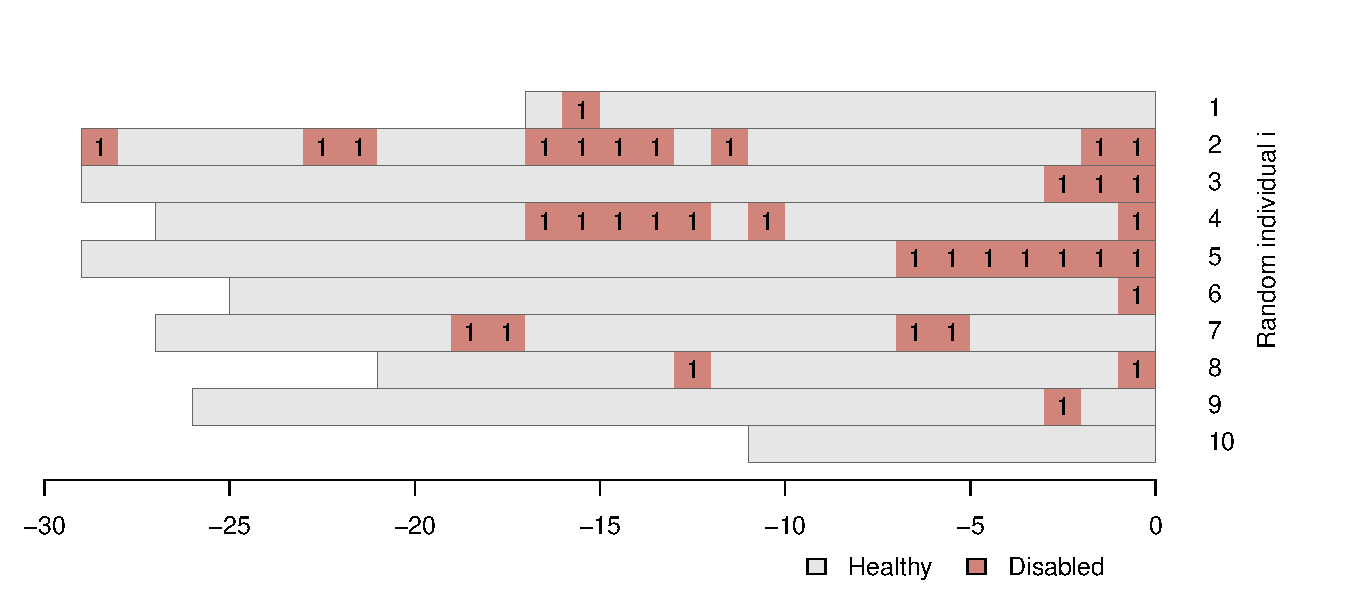
\includegraphics[scale=.45]{Figures/App1_grammar3.pdf}
    \caption{A prevalence clock, with trajectories aligned on the year of death. Healthy years are interpreted as 0s.}
    \label{fig:a1g3}
    \end{subfigure}
    \caption{Ten example disability trajectories. Figs. a) and b) indicate clock operations, and Fig. c) shows an alignment operation with a binary prevalence clock. Ages below 50 are ignored in these illustrations.}
    \label{fig:a1traj}
\end{figure}

To aggregate macro patterns from the spell duration and order clocks (Figs.~\ref{fig:a1g1} and \ref{fig:a1g2}, we calculate conditional means within each age, throwing out any values that are not the first time step in a disability spell. In the time-to-death prevalence we calculate conditional means within the time scale produced by death-alignment. In these examples, only individuals deceased before age 80 are shown, but in the full simulated sample some individuals reach age 80 in a state of disability, which may continue into higher ages if we had the transition probabilities to simulate so far. This introduces a downward bias in spell duration that grows in magnitude with the approach to age 80. For this reason, we right truncate results for spell duration aggregates at age 70. 

\FloatBarrier

\subsubsection{Results}
For each of the three variants, we calculate two age patterns, one for the highest and one for the lowest income quintile. One could potentially live 64 years between age 16 and 79, and survival for both income quintiles is close to complete. However, the higher income quintile spends on average 4 years disabled, whereas the lower income quintile spends 8.4 years disabled. Is this due to longer or more frequent bouts of disability? Are these bouts spread over life randomly, or concentrated toward the end?

Fig.~\ref{fig:a1m1} shows the results of aggregating trajectories coded as in Fig~\ref{fig:a1g1} by taking conditional means within single year age intervals. New disability spells are expected to be of longer duration as age increases. Disability spells are considerably longer on average for women in the lowest income quintile. From such an aggregate picture, a researcher could make various kinds of summary statements: at age 60, new disability spells for the poor are expected to be 40\% longer than for the rich. Or one could make statements on the age scale: new disability spells among the poor hit an average of two years duration by age 53, a level only hit by the rich around age 67.
\begin{figure}[ht!]
    \centering
    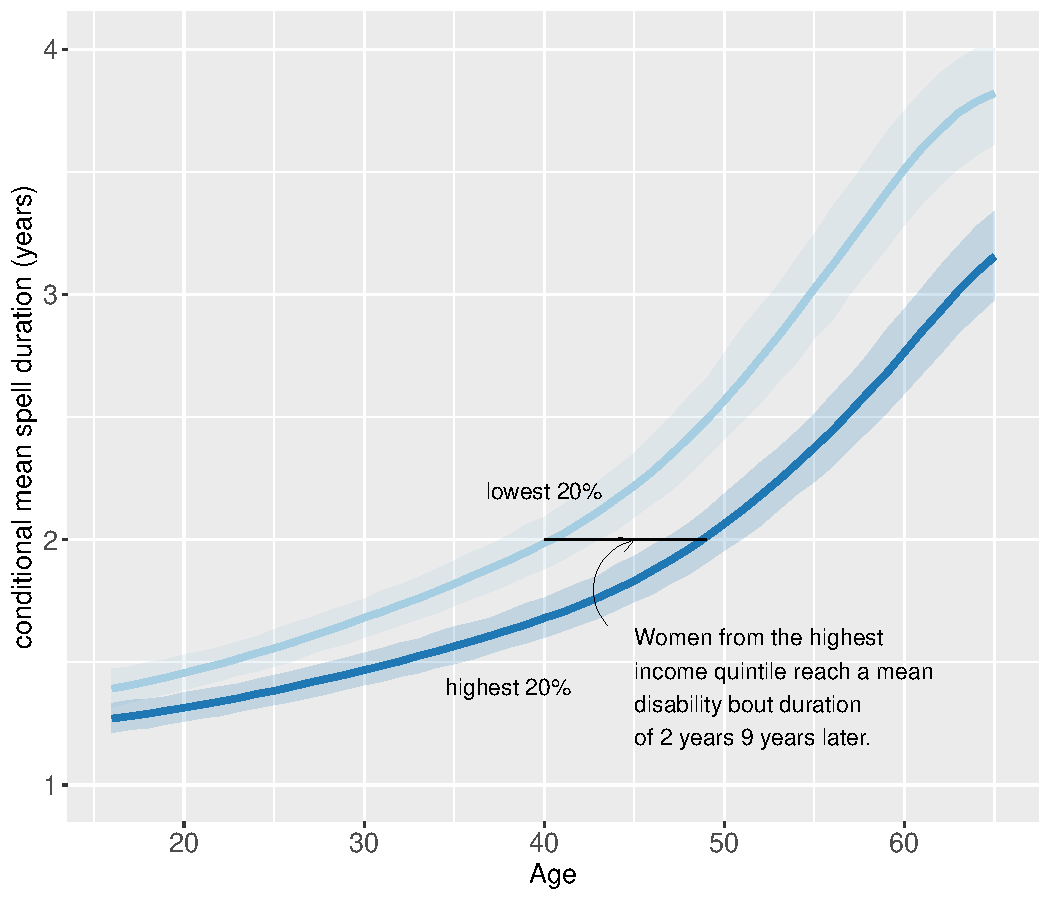
\includegraphics[scale=.6]{Figures/App1_macro1.pdf}
    \caption{Spells of disability get longer on average with age until at least age 70, and they are considerably longer on average for the lowest income quintile than for the highest. Mean duration of new spells passes two years at age 53 for the poor and age 67 for the rich.}
    \label{fig:a1m1}
\end{figure}

Fig.~\ref{fig:a1m2} shows the results of aggregating trajectories coded as in Fig~\ref{fig:a1g2} by taking conditional means within single year age intervals. We assume that everyone starts off having never been disabled before age 16, so anyone become disabled at age 16 is a first-timer. Some people recover and become disabled again at a later age, and for this reason new disability spells in higher ages are a mix of first and higher order bouts. In all ages after 20, individuals becoming disabled in the lowest income quintile have been disabled more often in their lives than those from the highest income quintile.
\begin{figure}
    \centering
    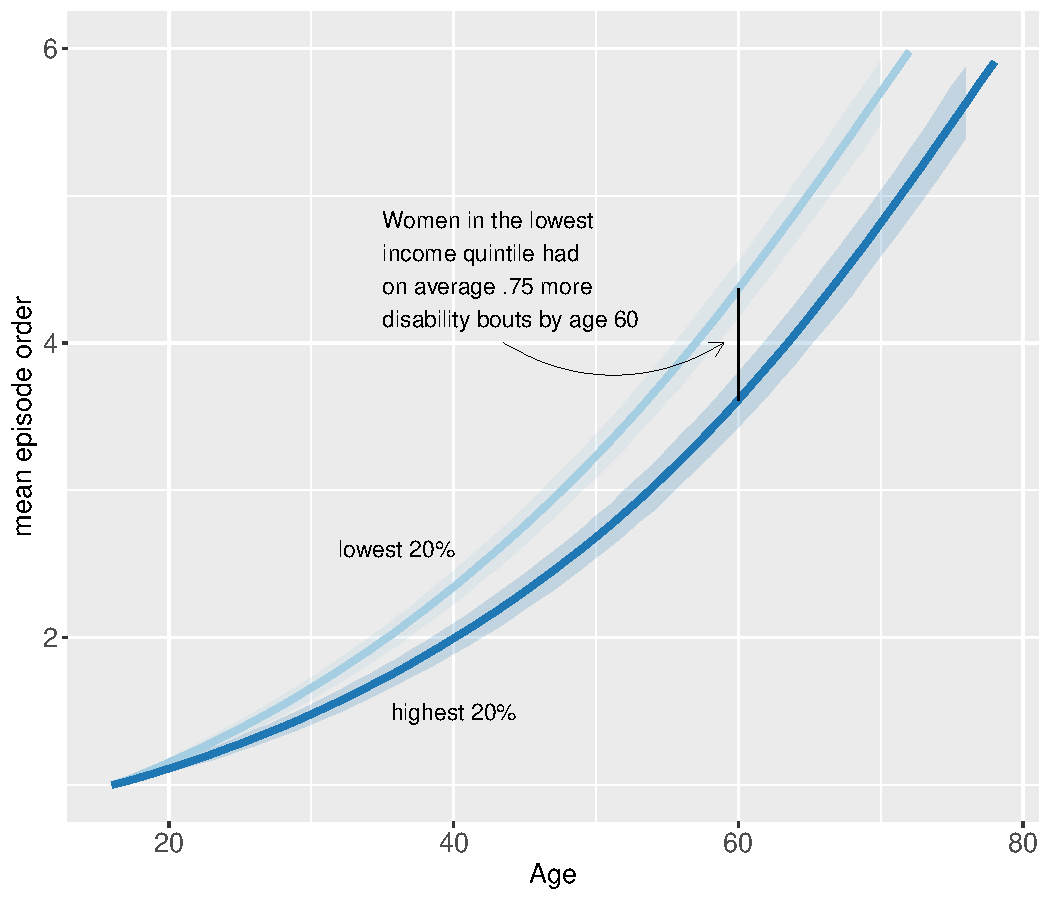
\includegraphics[scale=.6]{Figures/App1_macro2.pdf}
    \caption{The mean number of disability bouts of those experiencing disability increases with age faster for the lowest income quintile than for the highest.}
    \label{fig:a1m2}
\end{figure}

Fig.~\ref{fig:a1m3} shows the results of aggregating trajectories coded as in Fig~\ref{fig:a1g3}, where healthy years are coded as 0s and disabled years as 1s. We stratify the sample on 5-year groups by age of death to further demonstrate how the end-of-life pattern has a persistent shape. Lower ages at death are much noisier in this visualization because there are relatively few early deaths. This picture reveals two features of inequality: i) disability is more concentrated at the end of life for the highest income quintile, and ii) disability prevalence is consistently higher in all ages in the final third of life.

\begin{figure}
    \centering
    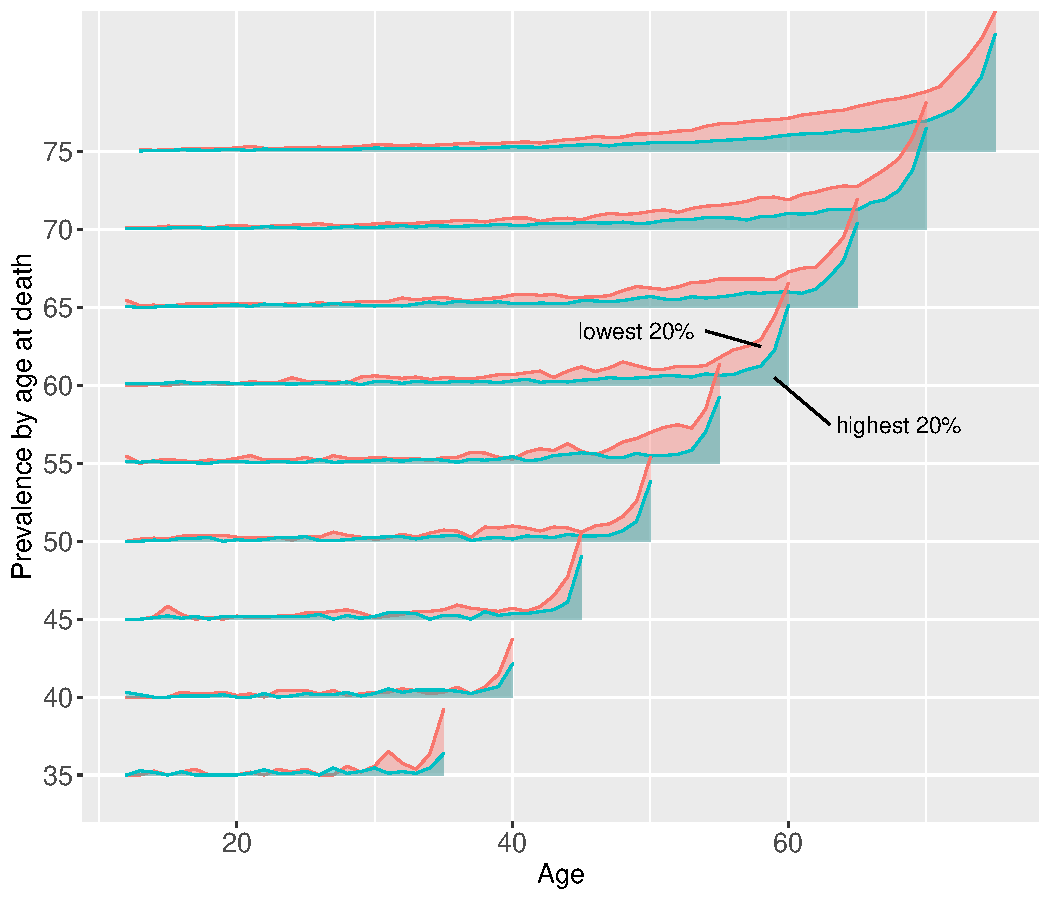
\includegraphics[scale=.6]{Figures/App1_macro3.pdf}
    \caption{The age pattern of disability prevalence is concentrated at the end of life. }
    \label{fig:a1m3}
\end{figure}

This stylized exercise evokes a number of follow-up questions that we do not here pursue: Are these pattern differences caused by onset, recovery, or mortality differences? Is this income gradient really a geographic gradient in disguise? How does this age pattern close out in ages higher than 80? Surely disability spell duration must start decreasing in higher ages when the force of mortality starts to dominate. In general, what fraction of disabled life expectancy is spent in short or long spells? What if we invert the analysis to examine healthy spells? Other clocks and alignments may reveal still other features of the health gradient in this domain of research.

\FloatBarrier
\subsection{Birth interval differentials}

 In our second application, we use this framework to examine the mean time to the second birth according to the sex of the first in Colombia from 1977 to 2010. We condition on the progression to second birth to reduce the influence of right-censored observations. The comparison of the mean time to second birth between women who had a daughter and women who had a son helps us answer the question of whether or not the sex of the first child increases the speed of transition to the second birth. 
 
  Although this is not a deep study of sex preferences in Colombia, we want to point out some background that would help to make sense of our results. Explicit practices of sex-discrimination at birth have not been documented in Colombia. In countries where sex-selective abortion is common, male live births outnumber female live births by more than 8\%, i.e., the ratio of male to females births is above 108. Colombia has a sex ratio at birth (SRB) that is considered 'normal' (around 105 boys per 100 girls) \cite{bongaarts2013}. Moreover, according to Fuse \citeyear{fuse2010}, 51\% of Colombian women in 2005 (ages 15 to 49) expressed they would like to have as many girls as boys (Balanced preference), 21\% said they would like to have more girls than boys (Daughter preference), and 13\% expressed a preference for sons. The remaining 15\% of women did not declare any gender preference. 
  %Second, according to the Colombian legislation abortion was illegal until 2006. A ruling of the Colombian Constitutional Court lifted the ban on abortion for three specific cases: (1) if mother's life is at risk, (2) if there is a malformation on the fetus that is incompatible with his/her life, or (3) if the pregnancy is the consequence of sexual abuse. However, legal abortions account for less than 1\% of . Third, it is important to bear in mind that the total fertility rate in Colombia declined  over the period of study. In 1987, the TFR was 3.2 children per women, and by 2010 it dropped to 2.1 (https://www.statcompiler.com).
 
  For these reasons, we expect small or no differences in the mean time to next birth according to the sex of the first child. There is no societal pressure on Colombian couples to have a son, and the share of women without gender preferences or balanced gender preferences is more than 65\%. Consequently the mean time to next birth should be independent of the sex of the first among couples with at least two children. However, the examination the mean time to second birth by sex of the first is a useful illustration of how to implement different clocks (time to next birth, time to next boy, and time to next daughter) and different alignments (timing of first birth by sex).
 
 
\subsubsection{Data}

We draw our data from six waves of the Colombian Demographic and Health Survey (CDHS) collected between 1987 and 2010 \citep{DHS}. The CDHS are nationally representative surveys of women in reproductive ages (15 to 49). We use full birth histories to reconstruct the reproductive trajectory of women with at least two children. We focus on women having their first birth within the ten years before the survey, and we measure the mean time to the second birth over the following eight years.

We are interested in the patterns of the mean time to second birth, mean time to next boy, and mean time to next girl. The starting point of our observation is, naturally, the year of the first birth. Using clocks and alignments, we are able to calculate the conditional mean time to second births diminishing the influence of right censoring, because all women in our sample had at least two children. 

Table \ref{tfert_01} shows the total number of women with at least two children according to the sex of the first birth and the year of the survey. 

\begin{table}[ht]
\centering
\begin{tabular}{lrrrrrrr}
  \hline
Sex of the  & \multicolumn{6}{c}{Period of reference} & Total \\
first birth & 1977-1987 & 1980-1990 & 1985-1995 & 1990-2000 & 1995-2005 & 2000-2010 & women \\ 
  \hline
Boy & 448 & 662 & 885 & 823 & 2402 & 2827 & 8047 \\ 
Girl & 455 & 615 & 796 & 795 & 2187 & 2565 & 7413 \\\hline 
Total & 903 & 1277 & 1681 & 1618 & 4589 & 5392 & 15460 \\ 
   \hline
\end{tabular}
\caption{Total number of women with at least two children ever born by sex of the first birth and survey year - Colombian Demographic and Health Surveys, 1987-2010}
\label{tfert_01}
\end{table}

Figure \ref{fert_illu} displays the fertility trajectory of 10 randomly selected women. The x-axis display women's age and the colors indicate when a birth occurred, and the sex of the newborn. Sequences have different lengths because women were interviewed at different ages. For example, the first women in this figure was 35 years old at the time of the survey and she had two children. The first child was a girl, born when the mother was 21. The second child was a boy, born when the mother was 27.

\begin{figure}[H]
\centering
    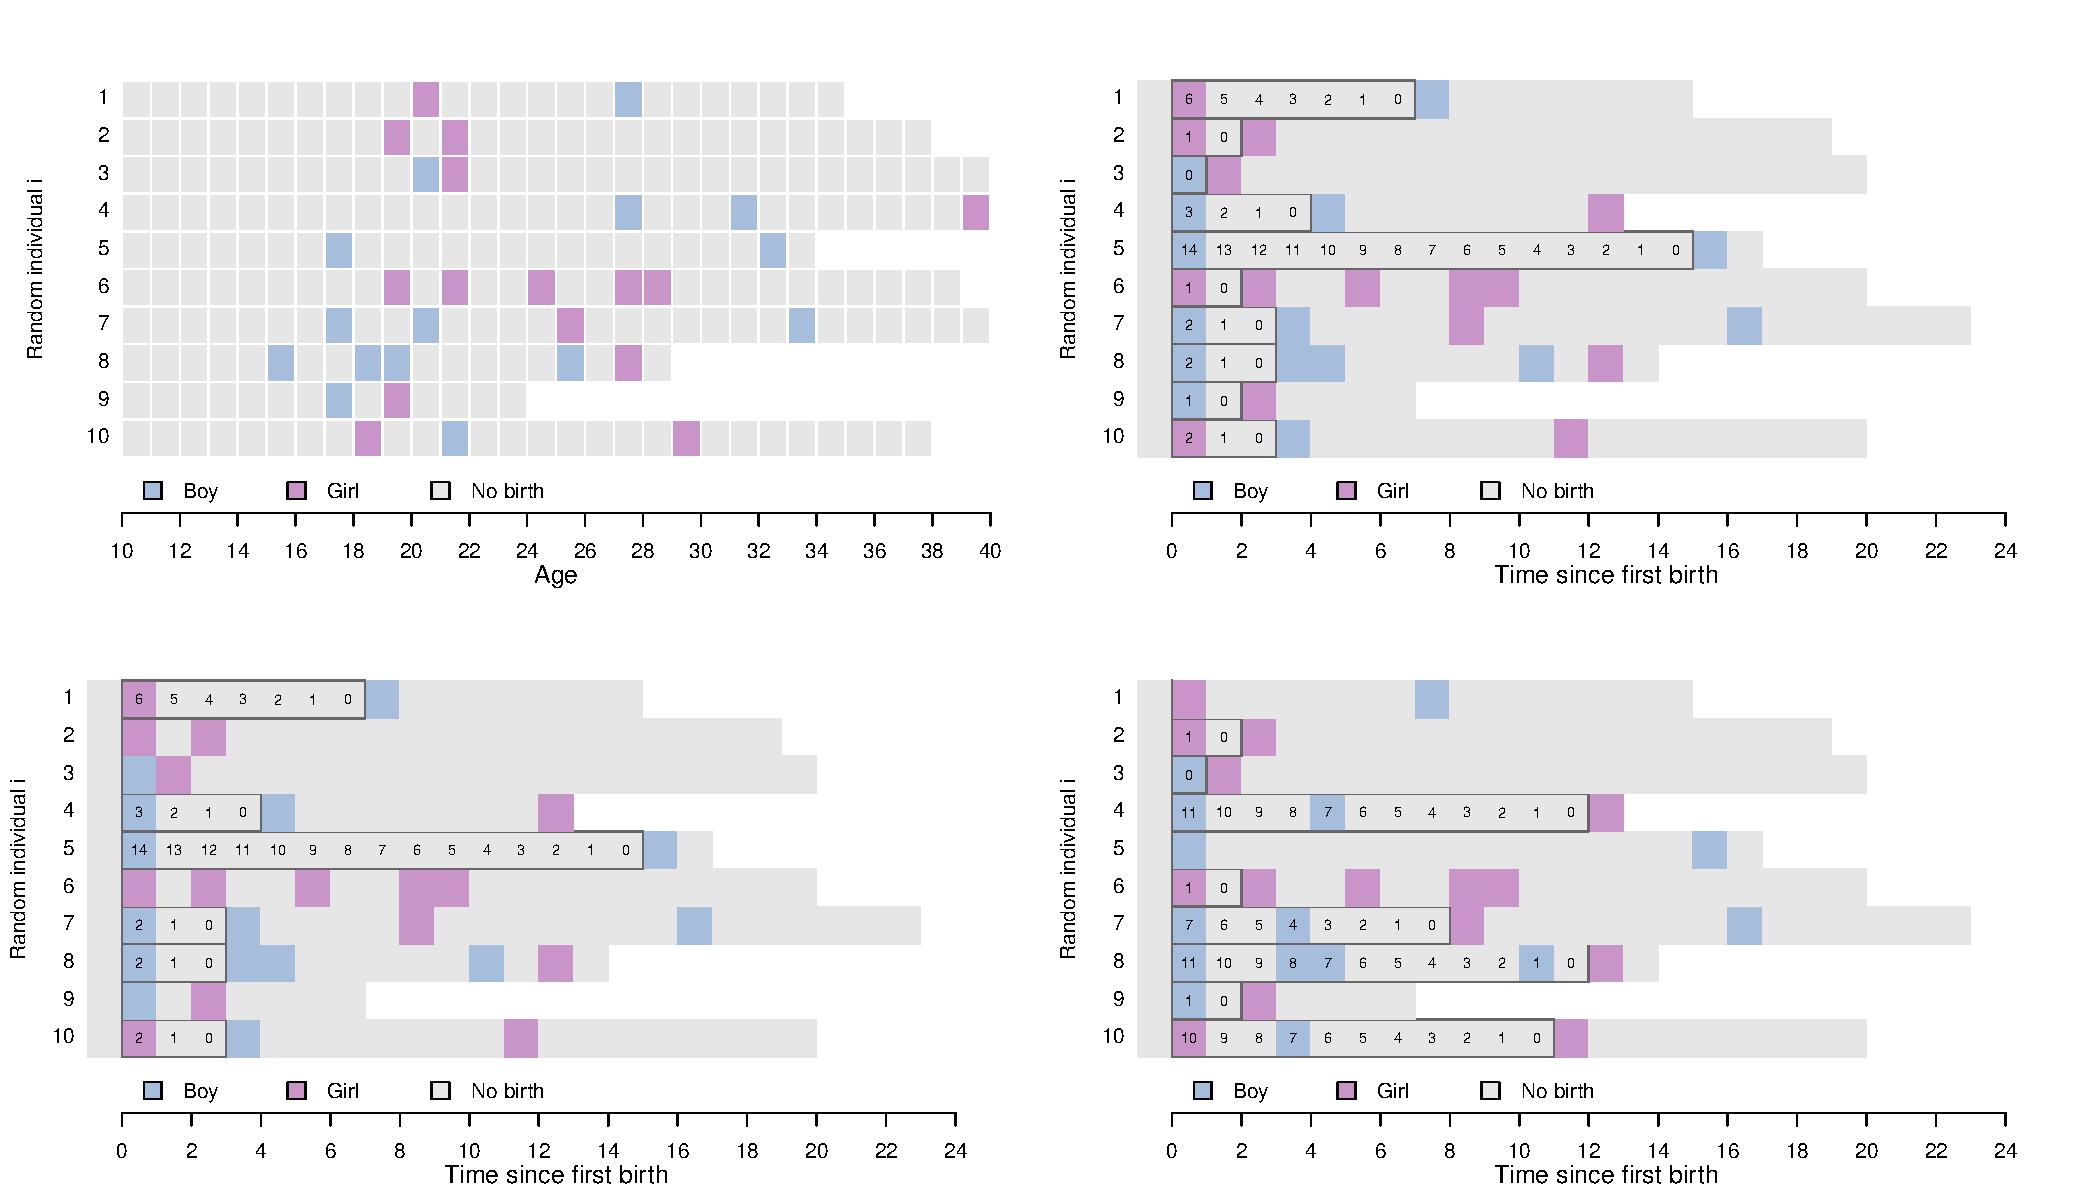
\includegraphics[trim=0cm 10cm 18cm 1cm, clip, width=0.95\textwidth]{Spells/Figures/colombia/illu_fertility.pdf}\\
    %\includegraphics[scale=0.8]{Spells/Figures/mt_second_birth_by_sex_first_cohort.pdf}
    \caption{Ten randomly selected fertility trajectories. Colombian Demographic and Health Surveys, 1987 - 2010}
    \label{fert_illu}
\end{figure}

In the first place, we are interested in the mean time to second birth, i.e., in the mean length of the spell between the first and second birth. Further we will explore the mean time to next boy and next girl. Note that these latter calculations are based on two different sub-samples, one for boys and one for girls. The sample for boys only includes women who had boys at parities above one (all women in Figure \ref{fert_illu} except numbers 2, 3, and 6), and the sample for girls only includes women with girls at parities above one (all women in Figure \ref{fert_illu} except numbers 1, and 5). %See detailed sample sizes in the appendix.


\subsubsection{Grammatical operations}

We use one alignment operation and three different clocks to get at the aggregate-patterns of mean time to second birth and mean time to next boy and girl. We align women's reproductive trajectory on the age at first birth. Figure \ref{fert_aling} displays the same ten sequences in Figure \ref{fert_illu} left-aligned according to first birth. The numbers in each trajectory count the years left to second birth, namely, a descending step clock to second birth. Naturally, the clock equals 0 the year before the occurrence of the second birth.\\

\begin{figure}[H]
\centering
    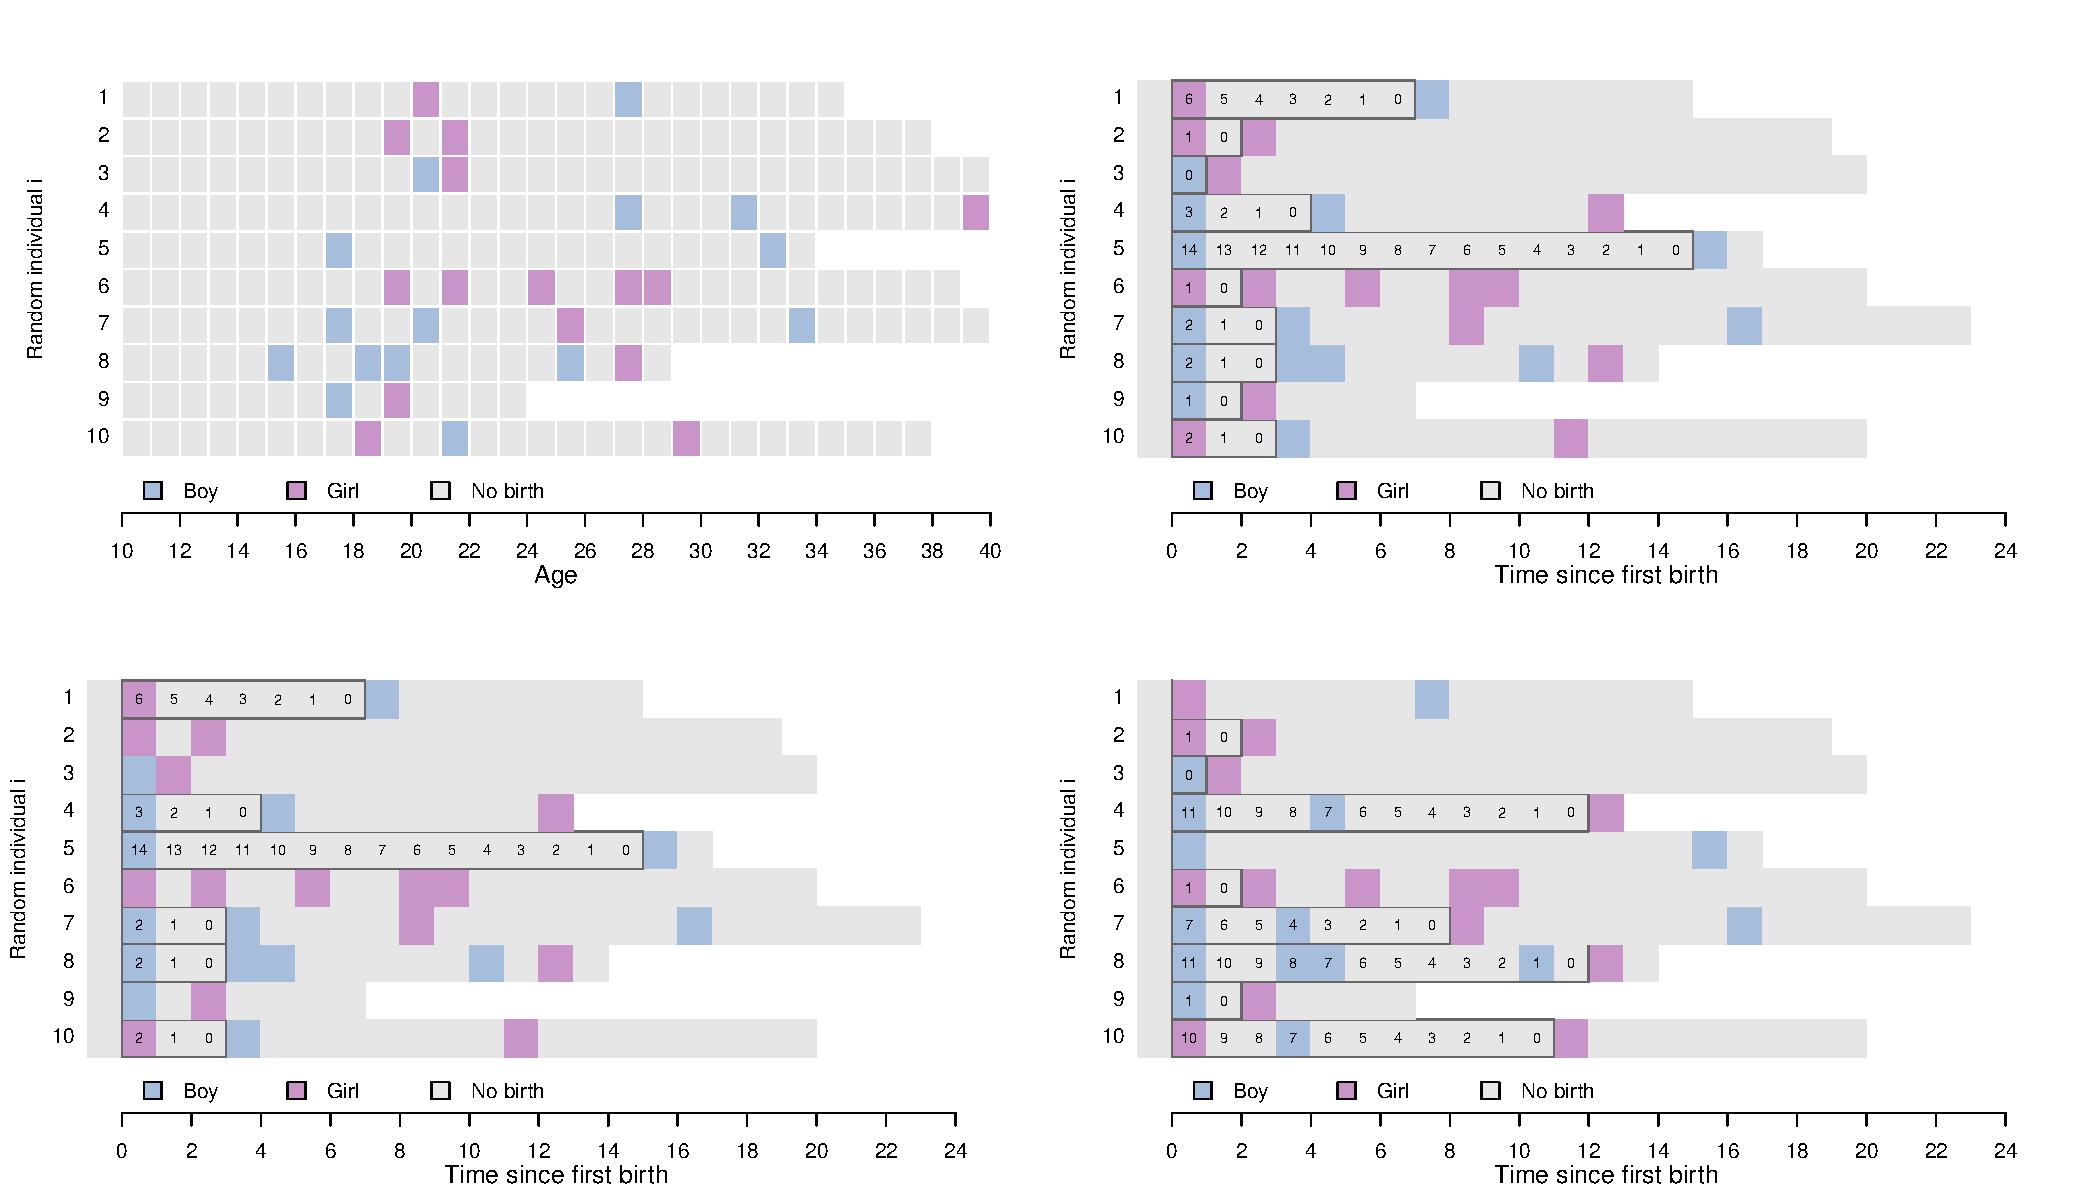
\includegraphics[trim=17cm 10cm 1cm 1cm, clip, width=0.95\textwidth]{Spells/Figures/colombia/illu_fertility.pdf}\\
    \caption{Descending step clock to second birth}
    \label{fert_aling}
\end{figure}

In Figure \ref{fert_aling}, the longest spell to second birth equals 14 years (women number 5). Whereas the shortest equals 1, for women 2 and 9. Once sequences are aligned and the numbers are assigned to the array, we compute column means to obtain mean time to second birth by duration since first birth. We separate women who first have a girl (sequences 1, 2, 6, and 10) and women who first have a boy (sequences 3, 4, 4, 7, 8 and 9).

We define two analogous clocks to examine differences by the sex of the second birth. In the first case, the clock counts the remaining years to the next boy (a descending step clock to next boy, Figure \ref{fert_clockb}); in the second case, the clock counts the remaining years to the next girl (a descending step clock to next girl, Figure \ref{fert_clockg}). 

\begin{figure}[H]
   \begin{subfigure}{\textwidth}
      \centering
   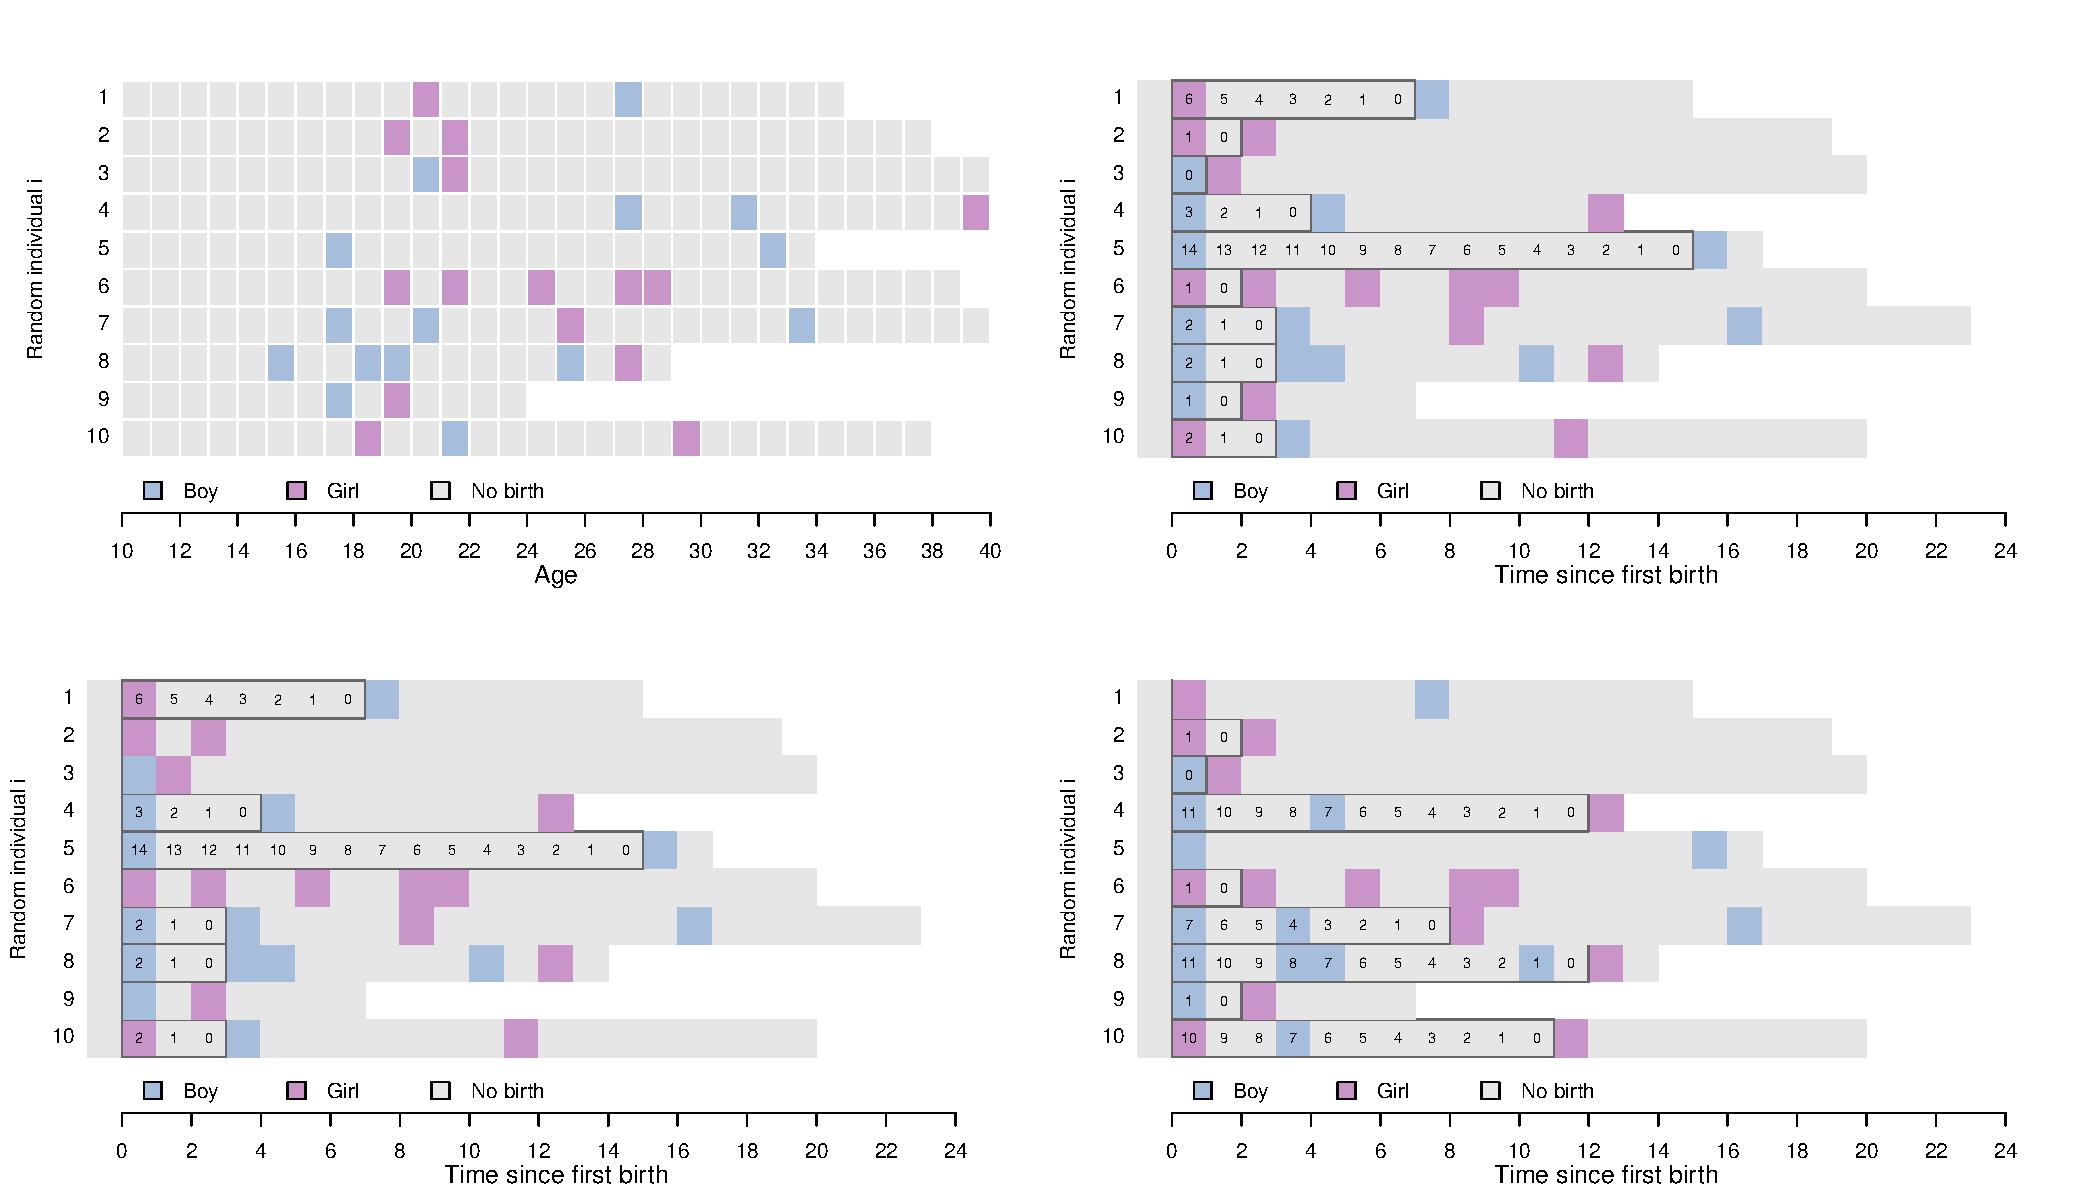
\includegraphics[trim=0cm 0cm 17.6cm 10cm, clip, width=0.95\textwidth]{Spells/Figures/colombia/illu_fertility.pdf}\\
    \caption{Descending step clock to next male birth}
    \label{fert_clockb}
    \end{subfigure}
    
       \begin{subfigure}{\textwidth}
      \centering
    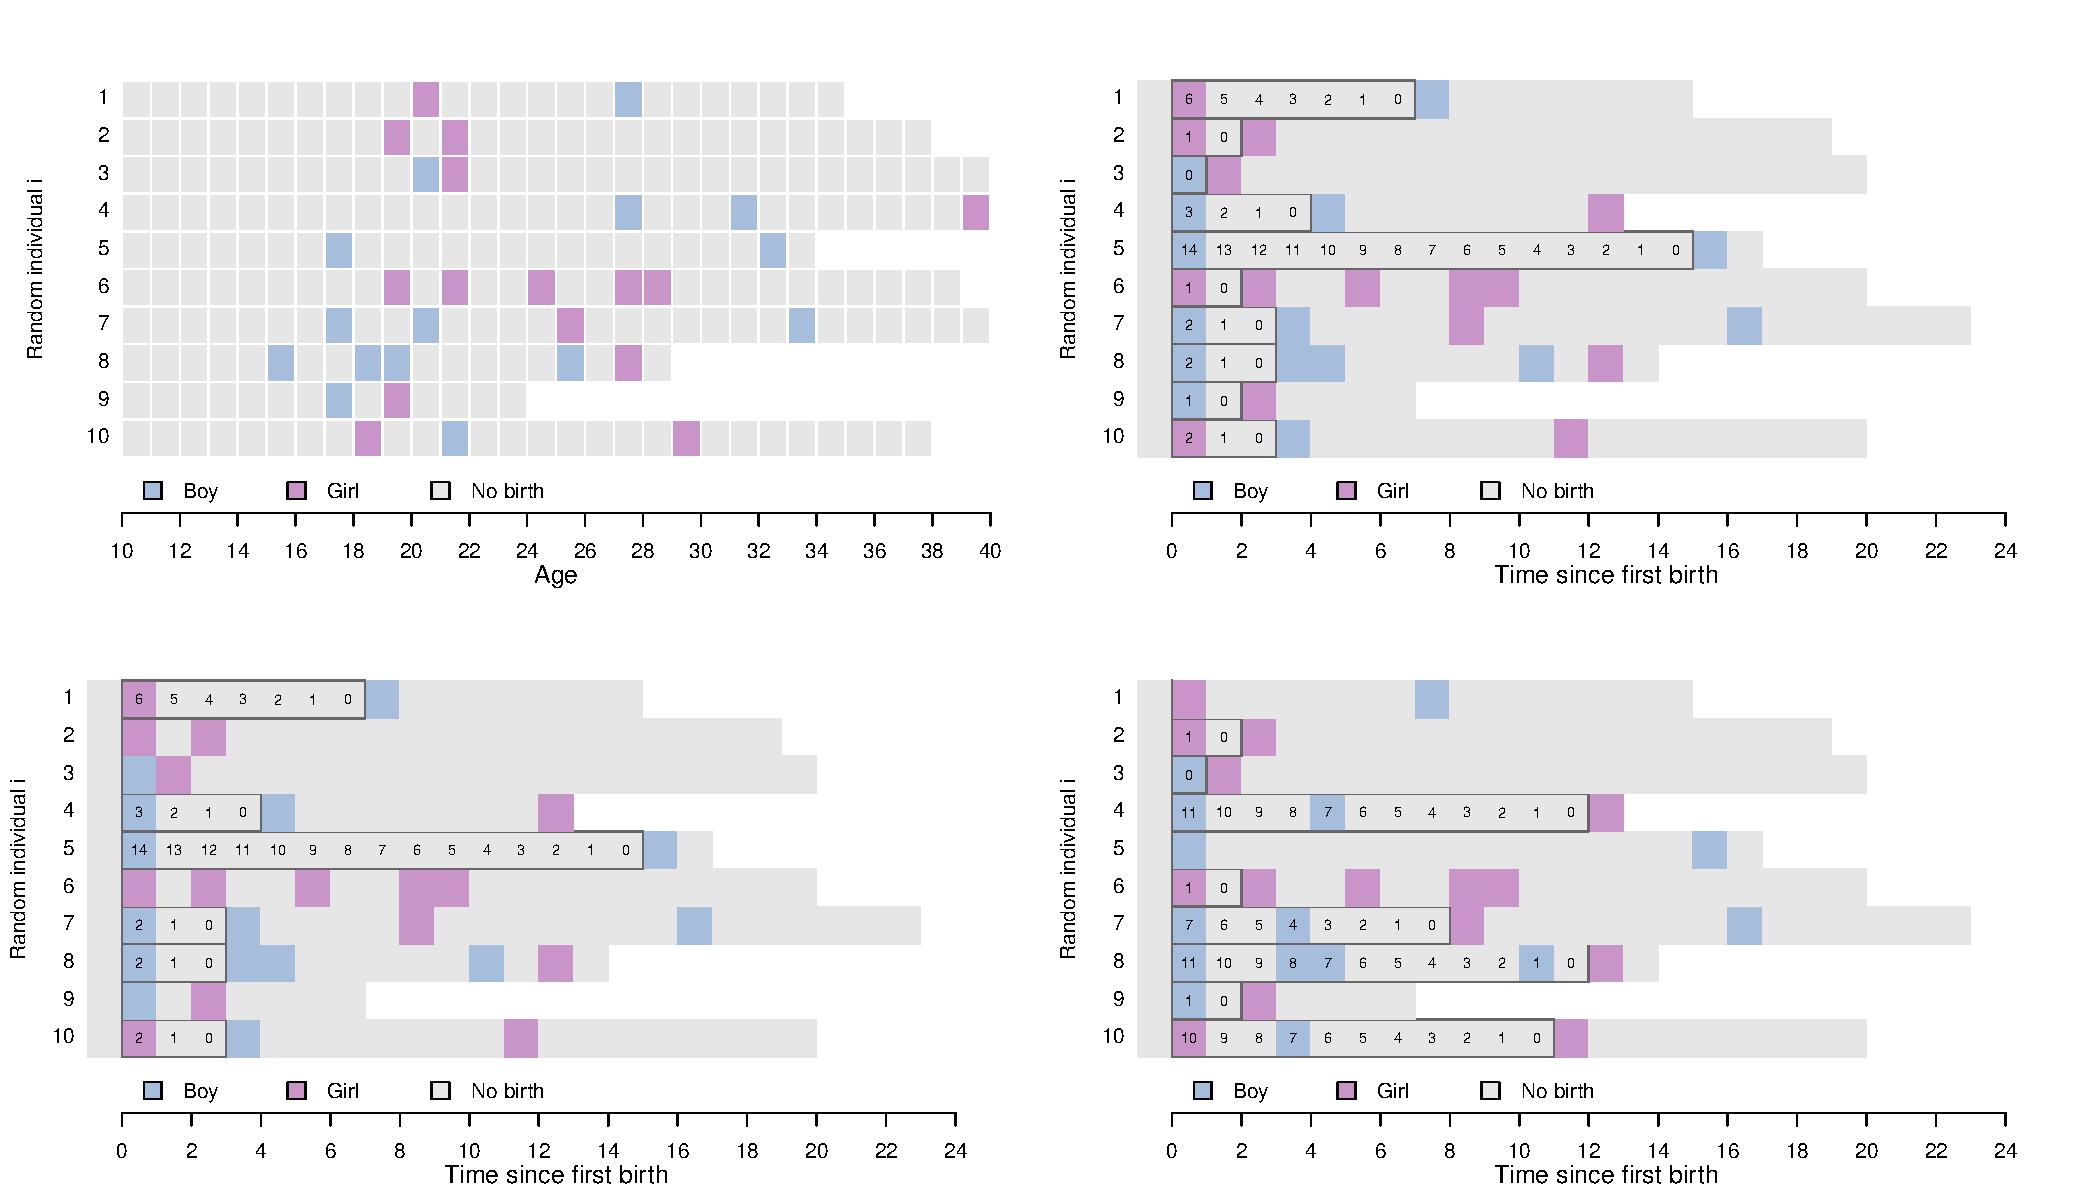
\includegraphics[trim=17.4cm 0cm 0cm 10cm, clip, width=0.95\textwidth]{Spells/Figures/colombia/illu_fertility.pdf}\\
    \caption{Descending step clock to next female birth}
    \label{fert_clockg}
    \end{subfigure}
    \label{fert_clock}
    \caption{Descending step clock to next birth conditional of sex of next birth}
\end{figure}

Note that these two clocks can only be defined if there is at least one boy and one girl after the first birth, respectively. This implies that the samples for the mean time to next boy and mean time to next girl are not identical. This difference between the samples is not problematic given the mere illustrative propose of our application. Moreover, clocks and sub-samples can be defined differently so that the two sample became identical, enhancing comparability.

\subsubsection{Results}
Figure \ref{fert_01} displays the aggregated patterns of the mean time to the second birth over the eight years after the first birth. Each panel corresponds to one CDHS from 1987 to 2010. The solid lines represent the median of 1,000 bootstrap replications of the sample mean, and the shaded area indicate the 2.5th and 97.5th percentiles of sample mean distribution. The width of the shaded areas reflect the level of uncertainty in the mean time to second birth. Overlapping areas between the sex-specific shaded areas indicate lack of statistical significance for the difference in the mean time to second birth according to the sex of the first. The gray rectangle of one year width indicate the birth of twins, i.e., mean time to next birth less than one year.
\begin{figure}[H]
\centering
    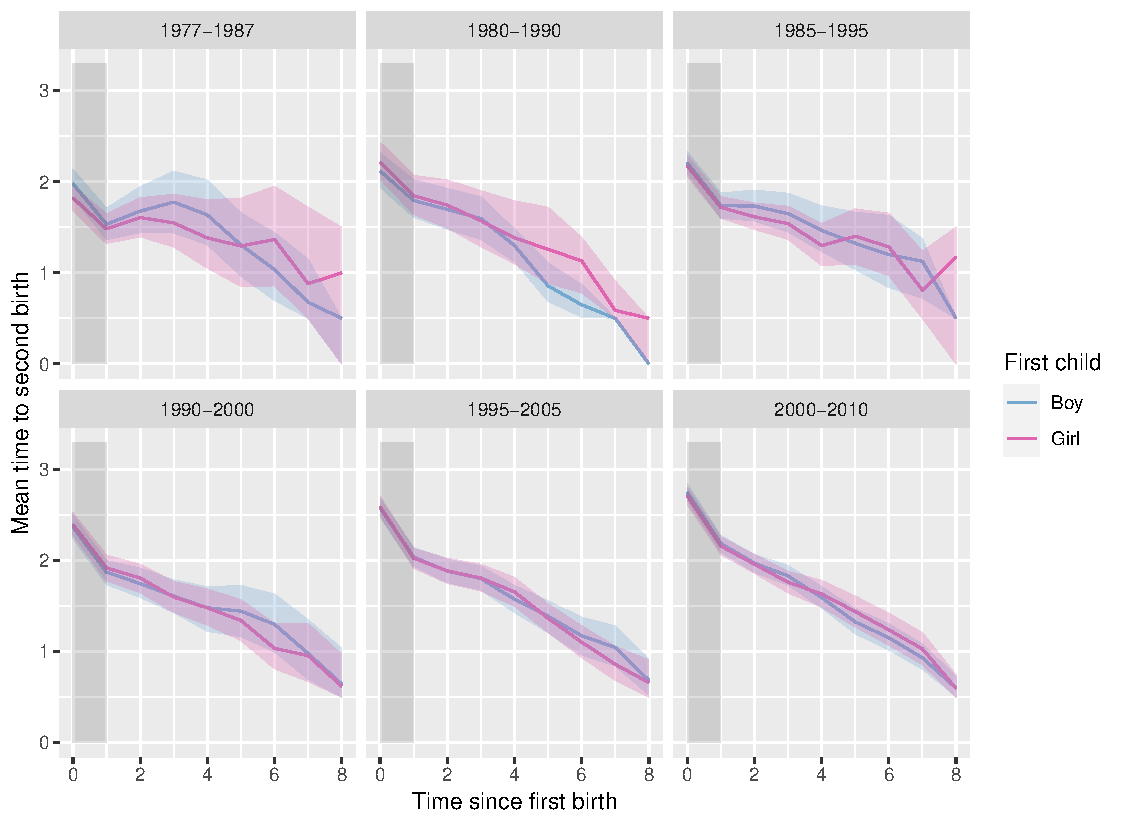
\includegraphics[width=\textwidth]{Spells/Figures/colombia/colombia_period_new_1.pdf}\\
    \caption{Median and uncertainty for the mean time to second birth by sex of the first in Colombia from 1977-2010}
    \label{fert_01}
 \end{figure}

Across surveys, the mean time to the second birth right after the first birth has increased from less than two years in 1987 to slightly more than 2.5 years in 2010, with a very narrow confidence interval. After the first year, the uncertainty of the mean time to next birth increases. These levels of uncertainty are larger in the first three surveys compared to the last three, mainly due to sample size. Finally, differences in the mean time to next birth by sex of the first child are never larger than one year, and the overlapping shaded areas indicate that they are not statistically significant.


Similar patterns appear when examining the mean time to next boy. According to Figure \ref{fert_02}, the sex of the first birth is not associated with shorter or longer intervals to next boy. 

Only for the 1977-1987 period, female first births are associated with a declining mean time to next boy starting at the second year after the first birth. By the fourth year since first birth, the mean time to next boy is below 1.5 years. In contrast, the mean time to next boy among women who had a male first birth stay around 2 years until the 4th year since first birth. Four years after first birth there is a statistically significant difference of more than six months in the mean time to next boy between first-time mothers of boys and first-time mothers of girls. 

\begin{figure}[H]
\centering
    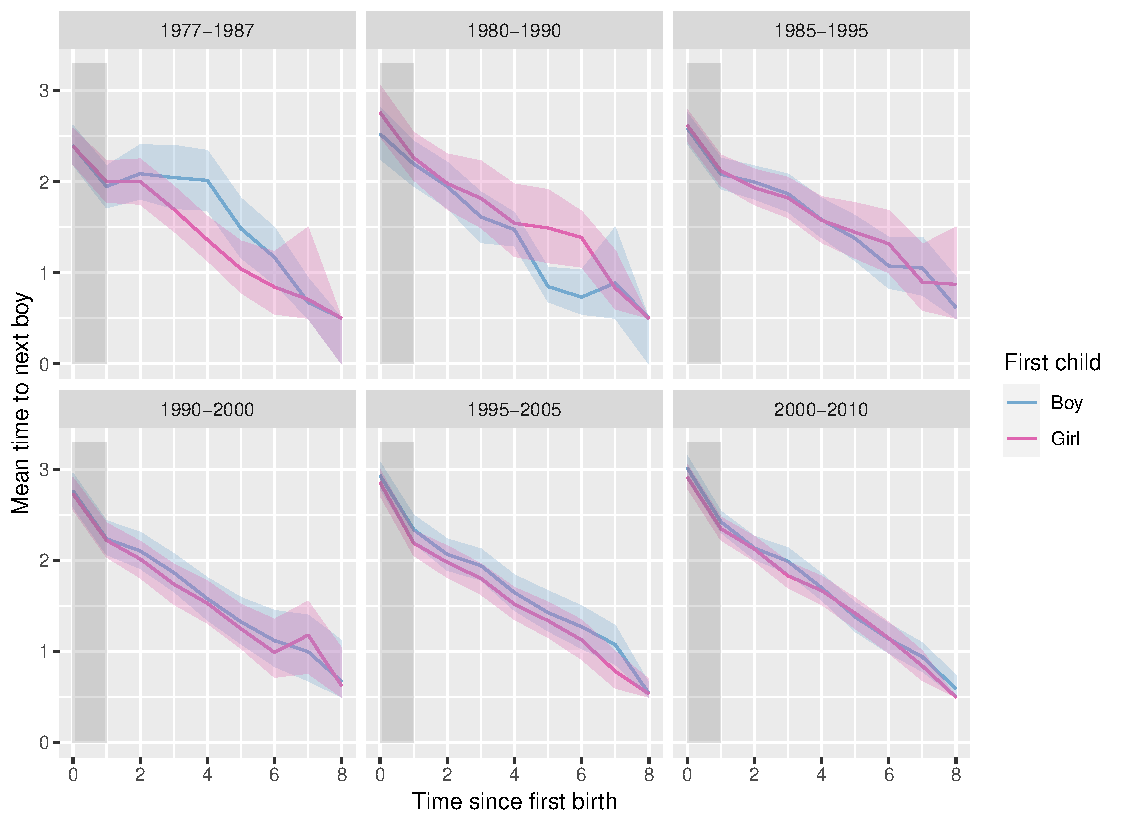
\includegraphics[scale=0.8]{Spells/Figures/colombia/colombia_period_new_2.pdf}\\
    \caption{Median and uncertainty for the mean time to next boy by sex of the first birth in Colombia from 1977-2010}
    \label{fert_02}
\end{figure}

This pattern is reversed in the the 1980-1990 period. Both, first-time mothers of boys and girls display declining mean times to next boy over the first four years since first birth; but this declining trend stabilizes for first-time mothers of girls, meaning that mothers of girls wait longer for the birth of a boy after the 4th year since first birth. After 1990, the mean time to next boy does not differ by sex of the first birth.

However, the overlapping patterns over the 8 years after the first birth across all other periods are a more robust and consistent pattern than these specific differences. The fact that sample sizes are particularly small for the first two periods (less than 700 women according to Table \ref{tfert_01}) make these results more subject to random variation compared to other periods where shaded areas are fully overlapped over the period of analysis.

Finally,  Figure \ref{fert_03} displays the patterns for the mean time to next girl. According to the 95\% confidence shaded areas, there are no statistically significant differences in the mean time to next girl by sex of the first birth in any of the surveys and at any point in time since first birth

\begin{figure}[H]
\centering
    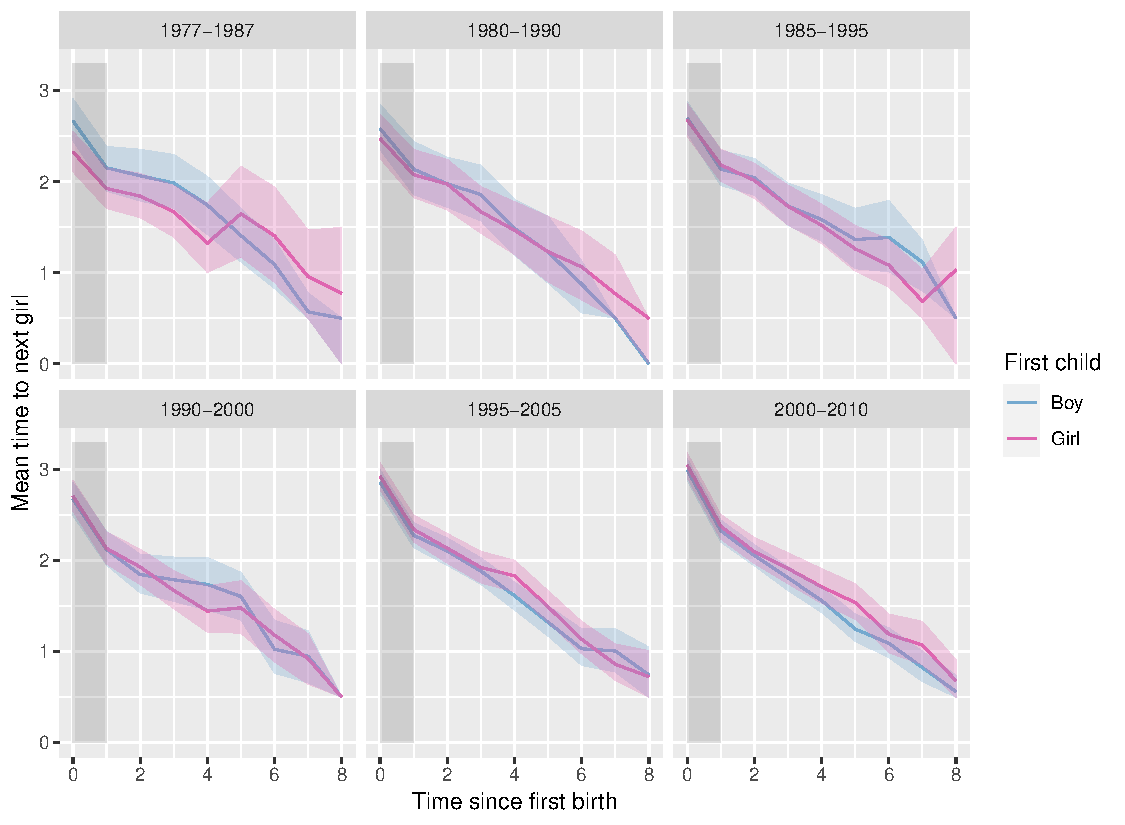
\includegraphics[scale=0.8]{Spells/Figures/colombia/colombia_period_new_3.pdf}\\
    \caption{Median and uncertainty for the mean time to next girl by sex of the first birth in Colombia from 1977-2010}
        \label{fert_03}
\end{figure}

These results are consistent with previous research that characterizes Latin American countries as places where there is negligible sex preferences, and therefore the timing of subsequent births is unaffected by the sex of previous births \cite{filmer2008}. Yet, much more detailed investigation of these patterns should be carried out before a robust conclusion can be derived. Meanwhile, this simple application has served us to show the flexibility of clocks and alignment to uncover patterns in fertility timing. There are several opportunities for applying this approach to countries where sex preference are stronger, and difference in timing by sex of the first birth could be more disturbed.

\section{Discussion}

We propose a two-part grammar of operations for life trajectory data to facilitate the creative derivation of demographic macro patterns. Our two applications for cases of birth interval differentials and disability inequalities demonstrate some of the flexibility and power of this grammar. Clocks and alignment operations, each have several potential variants. These operations may be executed separately or together for the same set of trajectories. We demonstrate clocks building from the simplest case of age-structured prevalence, and generalizing to a portfolio of yet-unexplored clock types. Some of these may already be familiar in specific contexts. For example birth parity would be considered an ascending order clock in our framework. Alignment operations are also already familiar in specific contexts, for example time-to-death patterns of morbidity or health expenditure constitute a right-alignment on the end of life \citep{riffe2017unified, raab2018pathways, potente2018disability}. Indeed, our disability example replicates the stylistic time-to-death prevalence patterns that have been directly observed in other populations \citep{klijs2010disability, riffe2016time}, and may serve as a demonstration of how age-structured multistate transitions can produce time-to-death prevalence patterns. We further generalize alignment operations by allowing for conditional alignment, for example on entry or exit from the first, last or longest episode of a given state.

We note two usage limitations on the application of alignments and clocks. First, aggregate measures based on clocks or alignment operations can be biased due to the left- or right-censoring of trajectories, i.e., when the observation window of sequences does not cover the full period over which events (change in states) can be observed. Our employment examples may be affected by left censoring because we do not know the employment status of individuals before age 50. To partially correct this, the data were simulated so that all individuals are employed by age 50, which makes mean calculations based on step clocks conditional on being employed at this age. Right censoring can be a problem for descending clocks (e.g., mean remaining time in a spell), especially at ages that are close to the end of the observation window (e.g. age 80 in our disability example below). Hence, researchers should be careful about the potential bias of the aggregate measures and make clear the conditional nature of them when necessary.

Second, care should be taken when conducting alignment operations as some observations will not be included in the aggregate measures if they do not experience the reference event for alignment. For example, individuals without spells of unemployment will not be included in the calculation of the mean time to next employment after a first job loss. Although these examples seem trivial, we encourage careful thinking when defining alignments, clocks, and aggregate measures.

The clocks and alignment framework was developed in order to accelerate experimentation with new macro patterns. Some of these operations might have tractable analogs when using Markov assumptions and matrix algebra approaches, albeit with the added overhead of needing to derive the required matrix expressions. Clocks and alignments could be fruitful post-processing steps to trajectories simulated from multistate transition probabilities. For the case of patterns derived from observed trajectories, as in our example of retrospective fertility histories, the results of such an exercise would also not be guaranteed to produce identical results as this framework. This is because the Markov approach is based on transition probabilities, which are not guaranteed to generate the same trajectory structure from which they were derived, whereas the clocks and alignment approach builds on this original structure. 

The data operations we describe are complementary to sequence analysis (SA), or may even be considered a subset of it. We speculate that alignment operations could be used within SA as a trajectory pre-processing step, and SA itself surely offers a host of applicable synthetic measures that could constitute clocks in our framework. Indeed, one of the inspirations to design this framework was a sequence analysis of disease states preceding death conducted by a peer scientist. This exercise was frustrated and abandoned due to heterogeneity in length of life but a methods constraint for trajectories to be of equal length. Alignment on end of life, and truncation to the $N$ preceding years would then allow for a variety of sequence clustering algorithms. This is essentially the exercise of \citet{potente2018disability} and \citet{raab2018pathways}. We hope our expanded set of alignment variants facilitates more diverse and flexible pattern detection of this kind.

The purpose of episode clocks and trajectory realignment is to detect important patterns in data (or model results) that are likely to otherwise go unnoticed. Some speculative heuristics about where to find such patterns might include that (i) life course events condition each other; (ii) temporal proximity to life course transitions is likely to be an important predictor of other transitions; (iii) within-episode patterns of other characteristics might be monotonically increasing or decreasing, concave, or convex. Aggregate patterns derived after such operations may be sharper and of more obvious interpretation and consequence than are age patterns. We think that this simple grammar has the potential to stimulate new questions and lead to new discoveries as well as better understandings of seemingly understood phenomena. Its generality is ensured by the provision of grammatical structure, which enables researchers to define new operations and further variants of clocks and alignments.


\section*{Acknowledgements}
This work has benefited from discussions with Christian Dudel, Erik Vickstrom, Marcus Ebeling, Jutta Gampe, Angela Carollo, and Maarten Bijlsma. 

\FloatBarrier
\singlespacing
\bibliographystyle{plainnat}
  \bibliography{references} 
\end{document}
